\documentclass [11pt,twoside]{article}
\usepackage[utf8]{inputenc}
\usepackage[T1]{fontenc}

%Page margins, header and footer positions
\usepackage{geometry}
 \geometry{
 a4paper,
 total={210mm,297mm},
 left=25mm,
 right=25mm,
 top=30mm,
 bottom=25mm,
 headsep=7mm}

\interfootnotelinepenalty=10000

%To display filling dots in the TOC for all entries
\usepackage[titles]{tocloft}
\renewcommand{\cftsecleader}{\cftdotfill{\cftdotsep}}

%Define new header and footer style
\usepackage{fancyhdr}

\pagestyle{fancy}
\fancyhf{}
\lhead{\color{Gray}{\small{SafeStreet Project - Maldini , Paone}}}
\lfoot{\textcolor{Gray}{\small{Copyright © 2019, Maldini, Paone – All rights reserved}}}
\rfoot{\textcolor{Gray}{\thepage}}
\renewcommand{\headrulewidth}{0pt}

%PACKAGES
\usepackage{wasysym}
\usepackage{pifont}

\newcommand{\supported}{\ding{52}\xspace}
\newcommand{\unsupported}{\ding{55}\xspace}
\newcommand{\partsupported}{\textcolor{black!40}{\ding{52}}\xspace}
\newcommand{\lowsupported}{\textcolor{black!20}{\ding{52}}\xspace}
\newcommand{\unknowsupported}{\textbf{?}\xspace}

%Font: Times
\usepackage{times}
%Change monospaced font
\renewcommand{\ttdefault}{lmtt}

%tables
\usepackage{tabu}
\usepackage{tabularx}
\usepackage{ltablex}
\usepackage{longtable}
\usepackage{float} % To allow the use of H modifier in long tables

%landscape mode
\usepackage{pdflscape}
\usepackage{rotating}
\usepackage{caption}

%make landscape mode be sensitive to even and odd pages
%start
\def\myrotate{\ifodd\c@page\else-\fi 90}
\makeatletter
\global\let\orig@begin@landscape=\landscape%
\global\let\orig@end@landscape=\endlandscape%
\gdef\@true{1}
\gdef\@false{0}
\gdef\landscape{%
    \global\let\within@landscape=\@true%
    \orig@begin@landscape%
}%
\gdef\endlandscape{%
    \orig@end@landscape%
    \global\let\within@landscape=\@false%
}%
\@ifpackageloaded{pdflscape}{%
    \gdef\pdf@landscape@rotate{\PLS@Rotate}%
}{
    \gdef\pdf@landscape@rotate#1{}%
}
\let\latex@outputpage\@outputpage
\def\@outputpage{
    \ifx\within@landscape\@true%
        \if@twoside%
            \ifodd\c@page%
                \gdef\LS@rot{\setbox\@outputbox\vbox{%
                    \pdf@landscape@rotate{-90}%
                    \hbox{\rotatebox{90}{\hbox{\rotatebox{180}{\box\@outputbox}}}}}%
                }%
            \else%
                \gdef\LS@rot{\setbox\@outputbox\vbox{%
                    \pdf@landscape@rotate{+90}%
                    \hbox{\rotatebox{90}{\hbox{\rotatebox{0}{\box\@outputbox}}}}}%
                }%
            \fi%
        \else%
            \gdef\LS@rot{\setbox\@outputbox\vbox{%
                \pdf@landscape@rotate{+90}%
                \hbox{\rotatebox{90}{\hbox{\rotatebox{0}{\box\@outputbox}}}}}%
            }%
        \fi%
    \fi%
    \latex@outputpage%
}
\makeatother
%end

%graphics
\usepackage{graphicx}
\usepackage[dvipsnames, table]{xcolor}
%If you upload images from PC, you need to insert code for the path here (different for Windows and Unix OS)

%References
%\usepackage{xpatch}
%\usepackage[backend=biber, style=numeric, citestyle=numeric, sorting=none]{biblatex}
%\addbibresource{main.bib}

%Other
\usepackage{ifthen}
\usepackage{xspace}
\usepackage{enumitem}
\usepackage{amssymb}
\usepackage[pdftex, colorlinks]{hyperref}
\newcommand{\comment}[1]{{\color{Red}$\blacktriangleright$ Comment: #1 $\blacktriangleleft$}}


% Some utilities\ldots
\usepackage{soul}
\usepackage{tikz}

\usetikzlibrary{calc}
\usetikzlibrary{decorations.pathmorphing}


\makeatletter

\newcommand{\defhighlighter}[3][]{%
  \tikzset{every highlighter/.style={color=#2, fill opacity=#3, #1}}%
}

\defhighlighter{yellow}{.5}

\newcommand{\highlight@DoHighlight}{
  \fill [ decoration = {random steps, amplitude=1pt, segment length=15pt}
        , outer sep = -15pt, inner sep = 0pt, decorate
       , every highlighter, this highlighter ]
        ($(begin highlight)+(0,8pt)$) rectangle ($(end highlight)+(0,-3pt)$) ;
}

\newcommand{\highlight@BeginHighlight}{
  \coordinate (begin highlight) at (0,0) ;
}

\newcommand{\highlight@EndHighlight}{
  \coordinate (end highlight) at (0,0) ;
}

\newdimen\highlight@previous
\newdimen\highlight@current

\DeclareRobustCommand*\highlight[1][]{%
  \tikzset{this highlighter/.style={#1}}%
  \SOUL@setup
  %
  \def\SOUL@preamble{%
    \begin{tikzpicture}[overlay, remember picture]
      \highlight@BeginHighlight
      \highlight@EndHighlight
    \end{tikzpicture}%
  }%
  %
  \def\SOUL@postamble{%
    \begin{tikzpicture}[overlay, remember picture]
      \highlight@EndHighlight
      \highlight@DoHighlight
    \end{tikzpicture}%
  }%
  %
  \def\SOUL@everyhyphen{%
    \discretionary{%
      \SOUL@setkern\SOUL@hyphkern
      \SOUL@sethyphenchar
      \tikz[overlay, remember picture] \highlight@EndHighlight ;%
    }{%
    }{%
      \SOUL@setkern\SOUL@charkern
    }%
  }%
  %
  \def\SOUL@everyexhyphen##1{%
    \SOUL@setkern\SOUL@hyphkern
    \hbox{##1}%
    \discretionary{%
      \tikz[overlay, remember picture] \highlight@EndHighlight ;%
    }{%
    }{%
      \SOUL@setkern\SOUL@charkern
    }%
  }%
  %
  \def\SOUL@everysyllable{%
    \begin{tikzpicture}[overlay, remember picture]
      \path let \p0 = (begin highlight), \p1 = (0,0) in \pgfextra
        \global\highlight@previous=\y0
        \global\highlight@current =\y1
      \endpgfextra (0,0) ;
      \ifdim\highlight@current < \highlight@previous
        \highlight@DoHighlight
        \highlight@BeginHighlight
      \fi
    \end{tikzpicture}%
    \the\SOUL@syllable
    \tikz[overlay, remember picture] \highlight@EndHighlight ;%
  }%
  \SOUL@
}

\makeatother

% Common abbrev. are set as commands to ensure proper spacing after the dot
\RequirePackage{xspace}
\newcommand{\ie}{i.e.\@\xspace}
\newcommand{\aka}{a.k.a.\@\xspace}
\newcommand{\Ie}{I.e.\@\xspace}
\newcommand{\cf}{cf.\@\xspace}
\newcommand{\Cf}{Cf.\@\xspace}
\newcommand{\eg}{e.g.\@\xspace}
\newcommand{\Eg}{E.g.\@\xspace}
\newcommand{\etal}{et al.\@\xspace}
\newcommand{\etc}{etc.\@\xspace}
\newcommand{\wrt}{w.r.t.\@\xspace}
\newcommand{\Wrt}{W.r.t.\@\xspace}



\date{}



\usepackage{eso-pic,graphicx}
\usepackage{float}
\usepackage[dvipsnames]{xcolor}
    \usepackage{listings}

\usepackage{hyperref}
\hypersetup{colorlinks,breaklinks,linkcolor=black,urlcolor=blue}
\begin{document}

%TITLE PAGE

\begin{titlepage}




{\begin{table}[t!]
\centering
\begin{tabu} to \textwidth { X[1.3,r,p] X[1.7,l,p] }
\textcolor{Blue}
{\textbf{\small{Computer science and engineering Software engineering 2 - Project 2019/2020}}} & 
\includegraphics[scale=0.5]{Images/PolimiLogo}
\end{tabu}
\end{table}}~\\ [7cm]


\begin{flushleft}




\end{flushleft}
\AddToShipoutPictureBG*{
\includegraphics[width=\paperwidth,height=\paperheight]{Images/SafeStreets.png}}
\end{titlepage}


\begin{table}[h!]
\begin{tabu} to \textwidth { X[0.3,r,p] X[0.7,l,p] }
\hline

\textbf{Deliverable:} & ITD\\
\textbf{Title:} & Implementation and Testing Document \\
\textbf{Authors:} & Maldini Pietro , Paone Angelo \\
\textbf{Version:} & 1.0 \\ 
\textbf{Date:} & 12-January-2020 \\
\textbf{Download page:} & https://github.com/pm390/MaldiniPaone\\
\textbf{Copyright:} & Copyright © 2020, Maldini Pietro, Paone Angelo – All rights reserved \\
\hline
\end{tabu}
\end{table}




\setcounter{page}{2}


%------------------------------------------------------------------------------------------------------------------------------------------------
\newpage
\addcontentsline{toc}{section}{Table of Contents}
\tableofcontents


%------------------------------------------------------------------------------------------------------------------------------------------------
\clearpage
{\color{Blue}{\section{Introduction and Scope}}}
\label{sect:introduction}

%---------------------------------------------------
\subsection{Purpose}
This document represents the Requirement Analysis and Specification Document (RASD). Goals of
this document are to completely describe the system-to-be in terms of functional and non-functional
requirements, analyse the real needs of the users in order to model the system, show the constraints
and the limit of the software and indicate the typical use cases that will occur after the release. This
document is addressed to the developers who have to implement the requirements and could be used as
a contractual basis. 
%---------------------------------------------------
\subsubsection{Goals}
\begin{itemize}
\item	USER:
\begin{itemize}
\item[G1] Notify authorities about traffic violations
\begin{itemize}
\item[G1-1] Send picture of violation
\item[G1-2] Send Position of the violation
\end{itemize}
\item[G2]Authorities must be able to take an available assignment
\item[G3] Allow authorities to report a finished assignment
\item[G4]Allow all actors to visualize update statistics
\item[G5] Allow the system manager to register Municipality to the service
\end{itemize}
\item	SafeStreets:
\begin{itemize}
\item[G6] Allow a Visitor to join the system registering him/herself to ensure reliability of the information provided by him/her
\item[G7] Store information about violations provided by users:
\begin{itemize}
\item[G7-1] Complete it with metadata
\item[G7-2] Mine information
\end{itemize}
\item[G8] Identify potentially unsafe areas:
\begin{itemize}
\item[G8-1] Suggest possible interventions
\end{itemize}
\item[G9] Allow municipality to register Authorities to the service
\end{itemize}
\item	Security Goals:
\begin{itemize}
\item[S1] Offer different levels of visibility to different type of users
\item[S2] Personal data of users are stored respecting current security standards
\end{itemize}
\end{itemize}
%---------------------------------------------------
\subsection{Scope}
\subsubsection{Description of the given problem}
SafeStreets is a crowd-sourced application whose intention is to notify the authorities when traffic
violations occur. Citizens, thanks to the system, will be able to send information about violations to the
authorities who will take actions against them. In this way, the service provided by the authorities can be
improved because they will receive notifications through the app. The sources of notifications are the
Citizens who take photos of violations and send them to the authorities through
the application. The information provided by users are integrated with other suitable information and are
stored by the service. The system also runs an algorithm to read the license plate of the vehicle in the
photos. All collected data can be seen by Citizens and authorities to find which streets are the safest.
Users can have different levels of visibility: authorities must be able to know the license plates of vehicles
in the photos, while normal users can only see data in the form of statistics. Moreover, data are sent to
the municipal district so that important information can be extracted through statistics in order to make
decisions to improve the safety of the area. Finally, the system will have to be easy to use, reliable
and highly scalable to fit perfectly with the mutable context in which it will be used.

%---------------------------------------------------
\subsubsection{Phenomena}
\begin{itemize}
\item
World phenomena:
\begin{enumerate}
\item
Violation
\item
Intervention of authorities
\item
Municipality put into effect interventions to improve safety
\end{enumerate}
\item
Machine phenomena:	
\begin{enumerate}
\item
Shortest path calculation for authority’s intervention (done by mapping system)
\item
the creation of an object of type violation
\item
run algorithm to identify the license plate/s in the photos
\item
schedule most efficient path to look up the notified violations
\item
periodically run algorithm to suggest possible interventions to municipality
\end{enumerate}
\item
Shared phenomena:
\begin{enumerate}
\item
user notify the system about violation (observed by the system controlled by the world)
\item
send notification to authorities (controlled by system observed by world)
\end{enumerate}
\end{itemize}
%---------------------------------------------------
\subsection{Definitions, Acronyms, Abbreviations}
\subsubsection {Definitions}
\begin{itemize}
\item	Violation: parking violations which can be notified by Citizens to authorities
\item	Report: Notification sent by Citizens to the system
\item	Mapping System: external software that provides maps and directions to reach the position of a violation
\item	Licence plate Recognition Algorithm: calculation process that identifies the alphanumeric number on license plate
\item	Spam: a series of messages that are undesired
\item	App: application software 
\item	Blocked: means that the account is banned for a given period
\item	Metadata: data about a violation. Position , date,  time and the username of Citizen. 
\item	Assignment : Work Request for authorities generated upon the receiving of a notification made by Citizens.
\end{itemize}
%---------------------------------------------------
\subsubsection {Acronyms}
\begin{itemize}
\item	RASD: Requirement Analysis and Specification Document.
\item	API: Application Programming Interface
\item	GPS: Global positioning system
\item	HTTP: HyperText Transfer Protocol
\item	HTTPS: HyperText Transfer Protocol over Secure Socket Layers
\item	UML: Unified Modeling Language

\end{itemize}
%---------------------------------------------------
\subsubsection {Abbreviations}
\begin{itemize}
\item	[Gn]: n-th goal.
\item	[Dn]: n-th domain assumption.
\item	[Rn]: n-th requirement.
\item     Municipality: municipal employee.
\end{itemize}
%---------------------------------------------------
\subsection {Revision History}
\begin{itemize}
\item      RASDv1.0 felivered on 10/11/2019: first delivery.
\item	RASDv2.0 delivered on 15/12/2019 : TODO write what we modified
\end{itemize}
%---------------------------------------------------
\subsection {Reference Documents}
\begin{itemize}
\item	Specification Document: “Assignments AA 2019-2020.pdf”.
\item	\href{http://homepage.cs.uiowa.edu/~tinelli/classes/181/Spring10/Notes/09-dynamic-models.pdf }{Alloy Dynamic Model example} 
\item	IEEE Std 830-1993 - IEEE Guide to Software Requirements Specifications.
\item	IEEE Std 830-1998 - IEEE Recommended Practice for Software Requirements Specifications.

\end{itemize}
%---------------------------------------------------
\subsection{Document Structure}
This chapter debates about contents and structure of RASD, indeed this document, based on standards IEEE, is divided in six different sections:
\begin{enumerate}
\item	The Introduction provides a general appearance of the systems defining which are the goals to reach, describing the problem and introducing the world and shared phenomena.
\item The Overall Description provides the description of the relevant components that system needs, the involved actors’ characteristics, and the assumptions to better clarify the needs and the boundaries of the system. 
\item Specific Requirements contains the goals, the functional and non-functional requirements of the system are presented. In addition, a mock-up representation of the application expslain and gives a feeling on how the app will look like and show the main actions it can perform.
\item Scenarios describe the usefulness of SafeStreet and its features in some situations that could happen.
\item UML Modelling contains the diagrams that are referred to the functionality of the system, they explain the workflow of some scenarios, the actions and the structure of the actors and the state that system assumes. These features are represented by Use Case diagram, Sequence diagram, Class diagram and Activity diagram.
\item Alloy Modelling allows to explain the world models through Alloy model of system. The mockups generated by the Alloy modelling grants that, given requirements and domain assumption, the goals are satisfied.

\end{enumerate}


%------------------------------------------------------------------------------------------------------------------------------------------------
\clearpage
{\color{Blue}{\section{Requirements and Functions}}}
\label{sect:Requirements and Functions}
%.-------------------------------------------------------------------------------------------------------------------------------------------------------------
\subsection{External Interface Requirements}
%.-------------------------------------------------------------------------------------------------------------------------------------------------------------
\subsubsection{User Interfaces}


\begin{figure}[h]
\centering
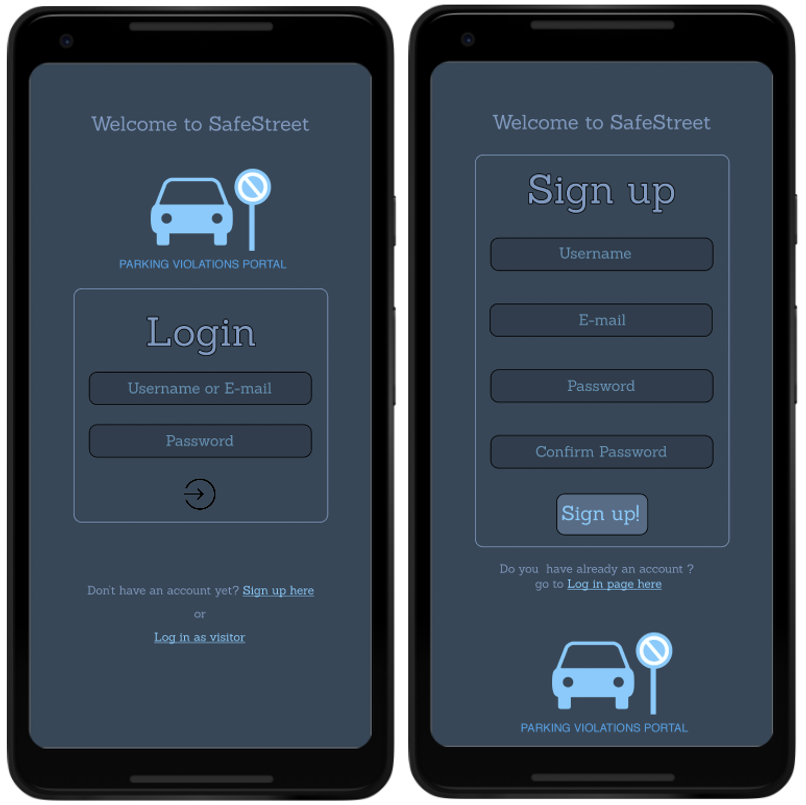
\includegraphics[width=\textwidth]{Images/login_signup.png}
\caption{\label{fig:ls}Login and Sign up }
\end{figure}

\begin{figure}[h]
\centering
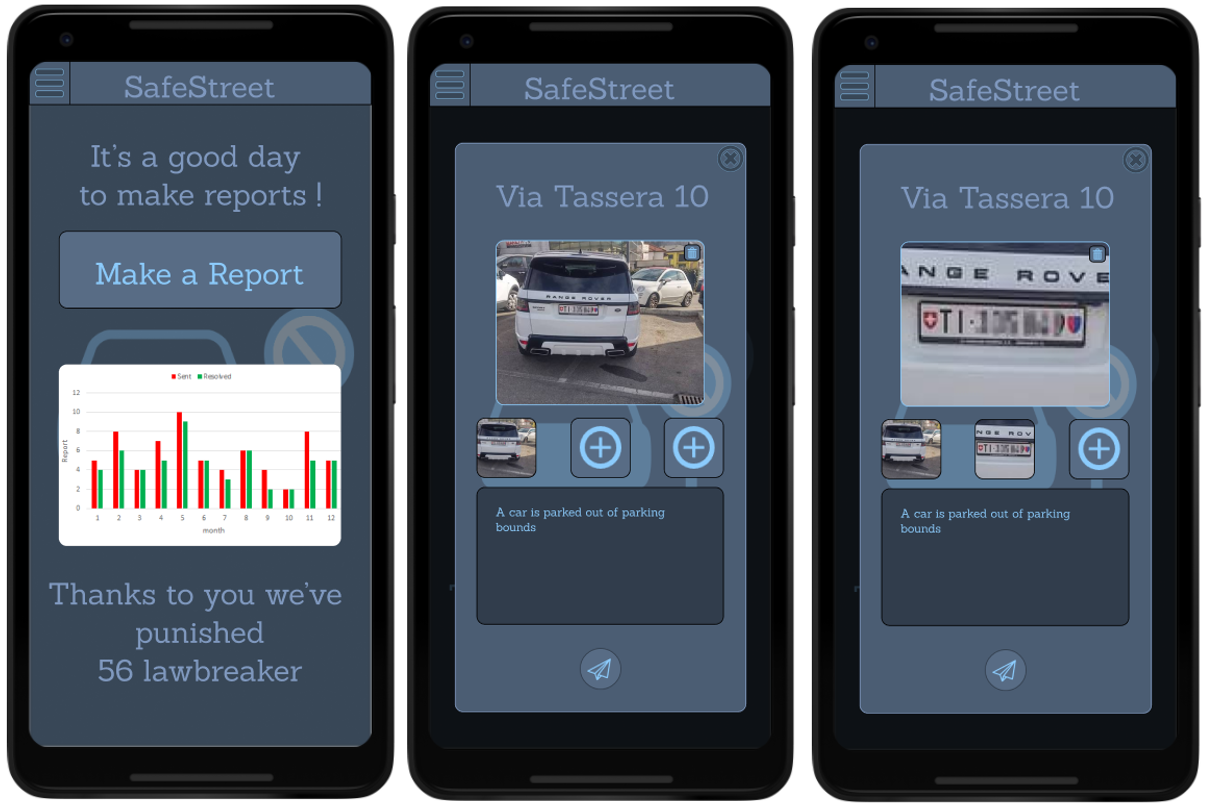
\includegraphics[width=\textwidth]{Images/user_interface.png}
\caption{\label{fig:CI}Citizen Interfaces}
\end{figure}

\begin{figure}[h]
\centering
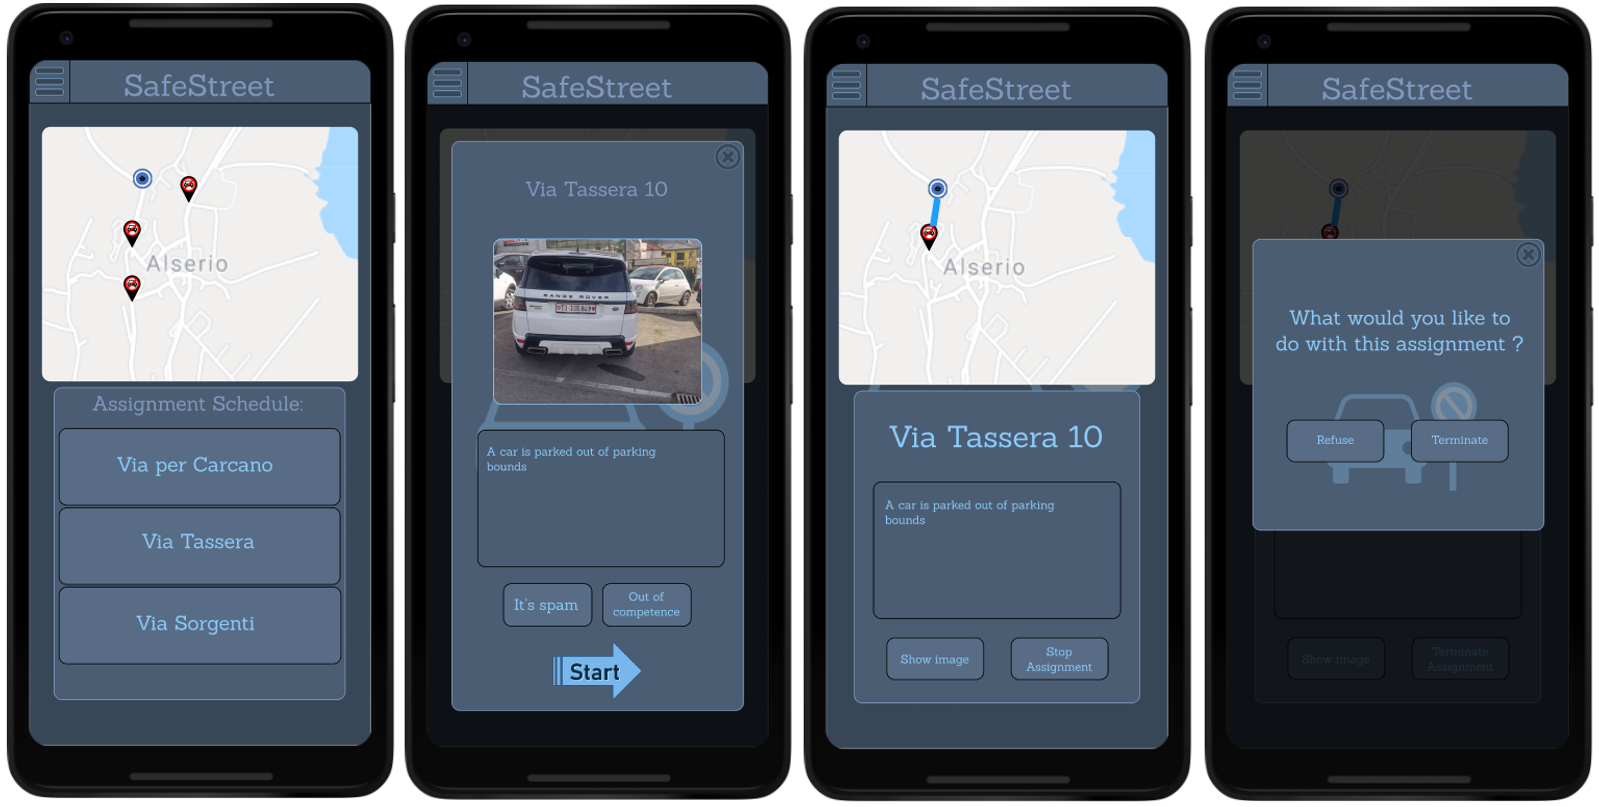
\includegraphics[width=\textwidth]{Images/agent_interface.png}
\caption{\label{fig:AI}Authority Interfaces }
\end{figure}

\begin{figure}[h]
\centering
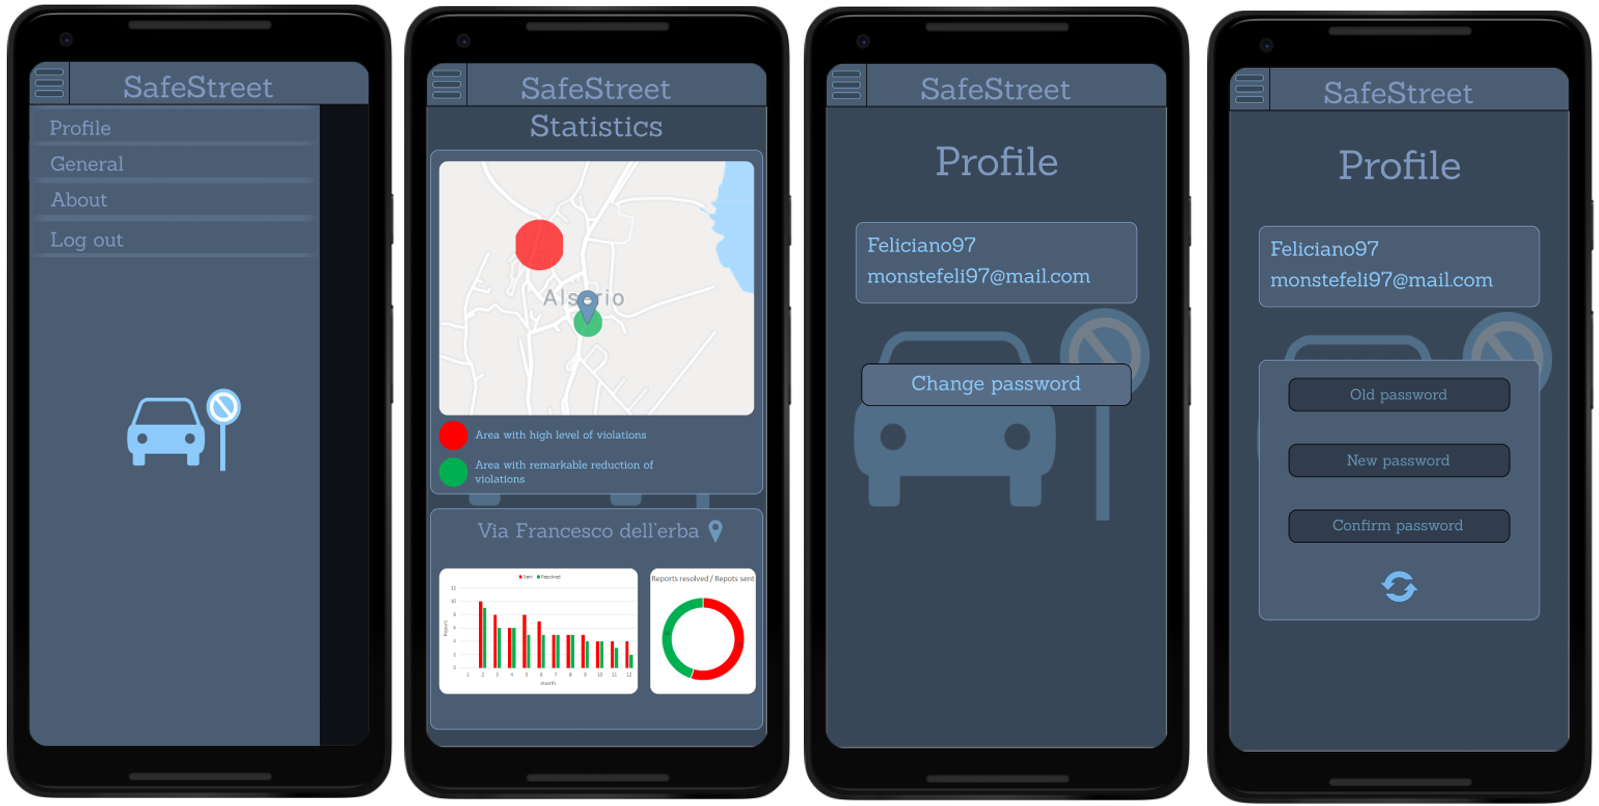
\includegraphics[width=\textwidth]{Images/common_interface.png}
\caption{\label{fig:ComI}Common Interfaces }
\end{figure}

\begin{figure}[h]
\centering
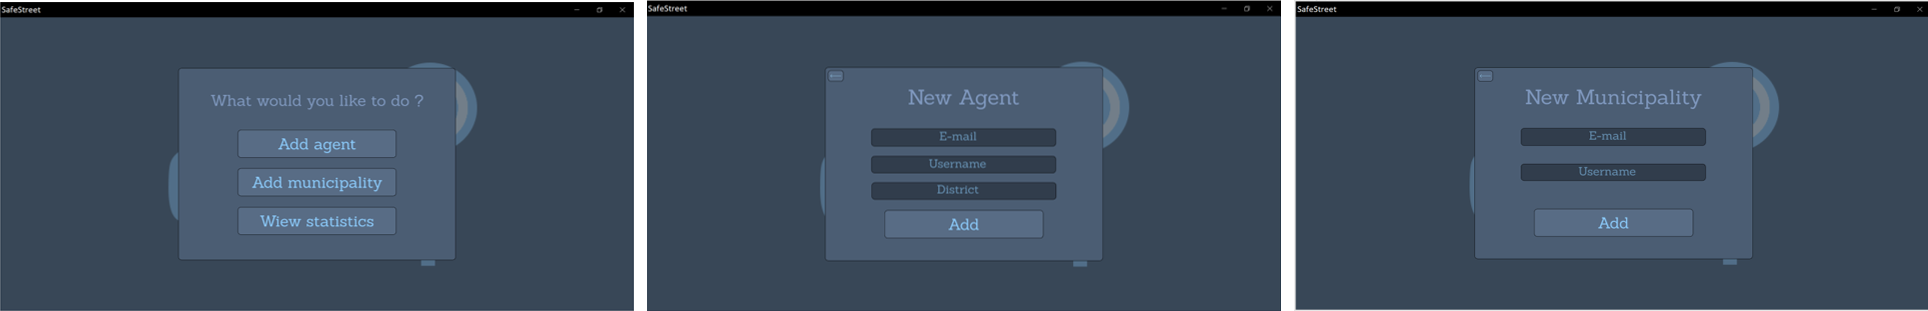
\includegraphics[width=\textwidth]{Images/municipality_interface.png}
\caption{\label{fig:MI}Municipality Interfaces }
\end{figure}

\begin{figure}[h]
\centering
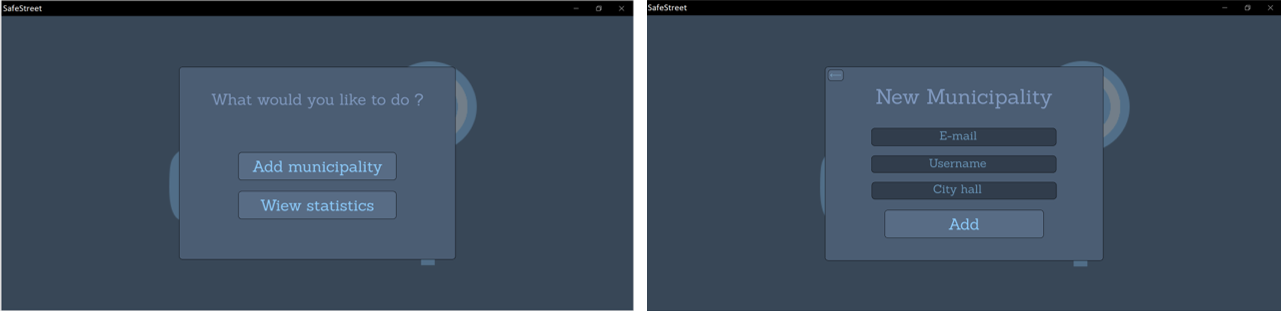
\includegraphics[width=\textwidth]{Images/system_manager_interface.png}
\caption{\label{fig:SMI}Sytem Manager Interfaces}
\end{figure}

\begin{figure}[h]
\centering
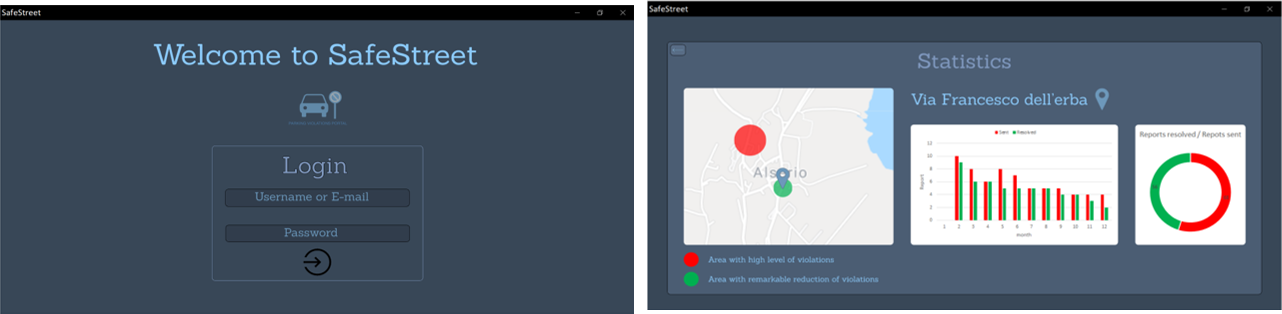
\includegraphics[width=\textwidth]{Images/desktop_common_interface.png}
\caption{\label{fig:ComWI}Common web Interfaces}
\end{figure}

%.-------------------------------------------------------------------------------------------------------------------------------------------------------------
\subsubsection{Hardware Interfaces}
There are no hardware interfaces to be implemented
%.-------------------------------------------------------------------------------------------------------------------------------------------------------------
\subsubsection{Software Interfaces}
Software interfaces to communicate with mapping systems, municipality databases and the algorithm to read Lisence plates are needed 
%.-------------------------------------------------------------------------------------------------------------------------------------------------------------
\subsubsection{Communication Interfaces }
To communicate the various internal parts of the S2B use HTTP and HTTPS protocol. No specific communication interface must be implemented.
%.-------------------------------------------------------------------------------------------------------------------------------------------------------------
\subsection{Functional Requirements}
\begin{itemize}

 \item R1) Authorities’ location must be known by the system when they are in service.
\item  R2) When a Citizen makes a report the position is correctly added with the GPS when is available.
\item R3) The right authorities are notified about violations.
 \item R4)  Authority must be able to provide the system how the assignment finished: resolved and the type of violation, no intervention needed when arrived, false report.
 \item R5) The system must make Statistics available when asked.
 \item R6) Statistics are always updated when an event happens.  
\item R7) For registering a Municipality his/hers data must be provided to a System manager who will add those data to the service to sign up him/her.
 \item R8) A visitor must be able to begin sign up process in the SafeStreets App filling a form with his data.
 \item R9) When the creation of an account is successful the system must notify the Visitor sending an email to the address provided in the sign up process. 
 \item R10) When GPS is not available the user can input the position from a map.
 \item R11) Users to use the full service must be able to login providing the right credentials.
\item R12) The camera of the mobile phone must be accessible to take photos of violations.
\item R13) Suggestions must be available when municipalities requests them.
\item R14) The User must be able to select the licence plate between the ones in output from the Licence Plate Recognition algorithm.
\item R15) Each Username is unique
\end{itemize}
%.-------------------------------------------------------------------------------------------------------------------------------------------------------------
\subsubsection{Scenrarios}
\begin{itemize}
\item Scenario 1:
\newline
Dimitri has an important appointment, but in front of his underground garage there is a car parked that doesn’t allow him to go out. He doesn’t know who the car owner is, so he can’t call him to move it. So, Dimitri decides to use Safestreet application: he takes a photo of the car, he adds the notes and he insert manually the position, because the GPS can’t take correctly the position, in order to send the violation to the authorities. After 10 minutes the public security agent, who has received the notification of Dimitri’s alert, arrives and means of removal take the car away and finally Dimitri can go to the appointment.


\item Scenario 2:
\newline
Angelo is the town councilman of Alserio. In the last period some citizen has alerted him that there are some people who park their car in the disabled parking near the Enigma café. They also have complained about the fact that there is not a public security agent to control the area. So, Angelo asks the mayor to use SafeSteets application in order to keep the violations under control. The mayor, enthusiast of his suggestion asks the system manager to add him into the service.After that, the mayor adds the other municipality employees, so they can add the authorities too.Therefore , thanks to the app , the authorities receive warnings about infractions in various part of the town and they can intervene. Moreover, thanks to the statistics supplied by the application, the mayor manages to start a policy of prevention of the violation.
\item Scenario 3
\newline
Manuel asks his friend Fred if he wants to join him for dinner this evening at his place. Unfortunately, Fred's car is blocked by a vehicle parked in front of his garage. He has noticed that car has been there several days in the past months. Since Fred works near his house, he goes to work by bike, but his friend lives far from his house, so he can't get there without his car. So, Fred decides to download SafeStreets app on his smartphone. He provides all the information required to the system in order to sign up; then he logs in and sends a notification to the authorities. One hour before leaving he notices that the car has been removed. From that day on the car owner stopped parking there.
\item Scenario 4:
\newline
Today in Milan there are lot of violations and the authorities can't check every one of them. After some time, the violations not assigned lose their priority and go down in the assignment list. Agent Carlo usually checks the areas between Milano Piola and Milano Lambrate. Lots of violations are notified by users in those areas. However, by the time he finishes checking some violations, other become less visible due to the great amount of notifications. When different users notify a violation concerning a license plate in the same area, this one becomes more visible in the assignment list. Thanks to this feature, Carlo is able to first address issues affecting more people.

\item Scenario 5:
\newline
Pietro is an agent who has just been employed in Alserio police; his method of street controlling is “old school” and a little bit disorganized, but his colleague Sonia recommends him SafeStreet application. So, Pietro goes to the town hall to register himself into the Safestreet database. The employee checks his credential and his work district, and the system sends him the transient credential.  Then, Pietro installs the app and uses the transient credentials in order to log into his personal page and change the credentials to confirm the account. Thanks to SafeStreet application, his job is now organized better because he can go to exact violations place.
\item  Negative Use Scenario 6:
\newline
Fernand got his car fined after having parked in a forbidden area. He has been doing it for years, but now he notices that people in that area started using SafeStreets app and thinks that he was fined because of it instead of his behaviour. He decides to "take revenge" subscribing to the app and sending several false notifications. Since he has sent several random photos without any visible licence plate, the system signs the assignments given by Fernand account as "possibly unsafe". After that some agents have checked that no violation is actually in any of the photos sent to the system, his account gets blocked and Fernand can no longer interfere with the normal activities of authorities using the app. After being blocked, Fernand stops complaining about the app and a week later he finds a parking area to replace his former parking spot.
\end{itemize}
%.-------------------------------------------------------------------------------------------------------------------------------------------------------------
\newpage
\subsubsection{Use Case Diagrams}
\begin{figure}[h]
\centering
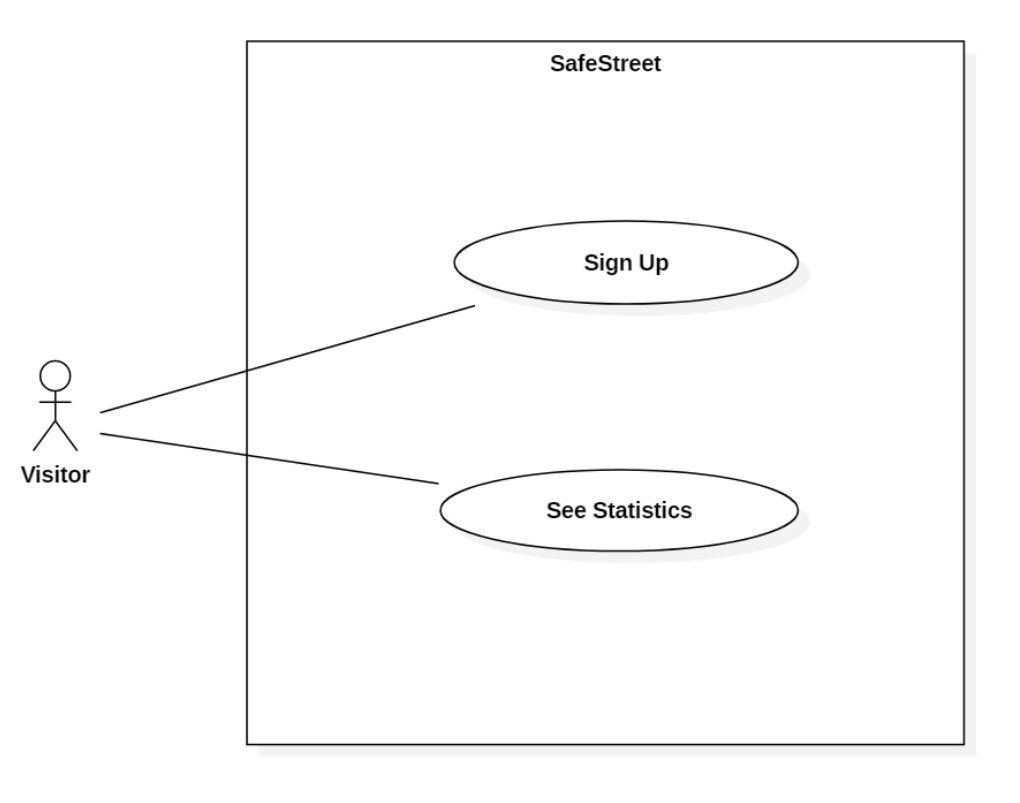
\includegraphics{Images/usecase_visitor.png}
\caption{\label{fig:VUC}Visitor Use Case }
\end{figure}
\begin{figure}[h]
\centering
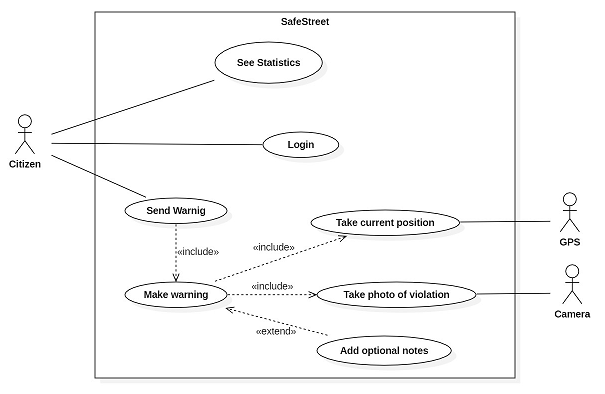
\includegraphics[width=\textwidth]{Images/usecase_citizen.png}
\caption{\label{fig:CUC}Citizen Use Case }
\end{figure}
\begin{figure}[h]
\centering
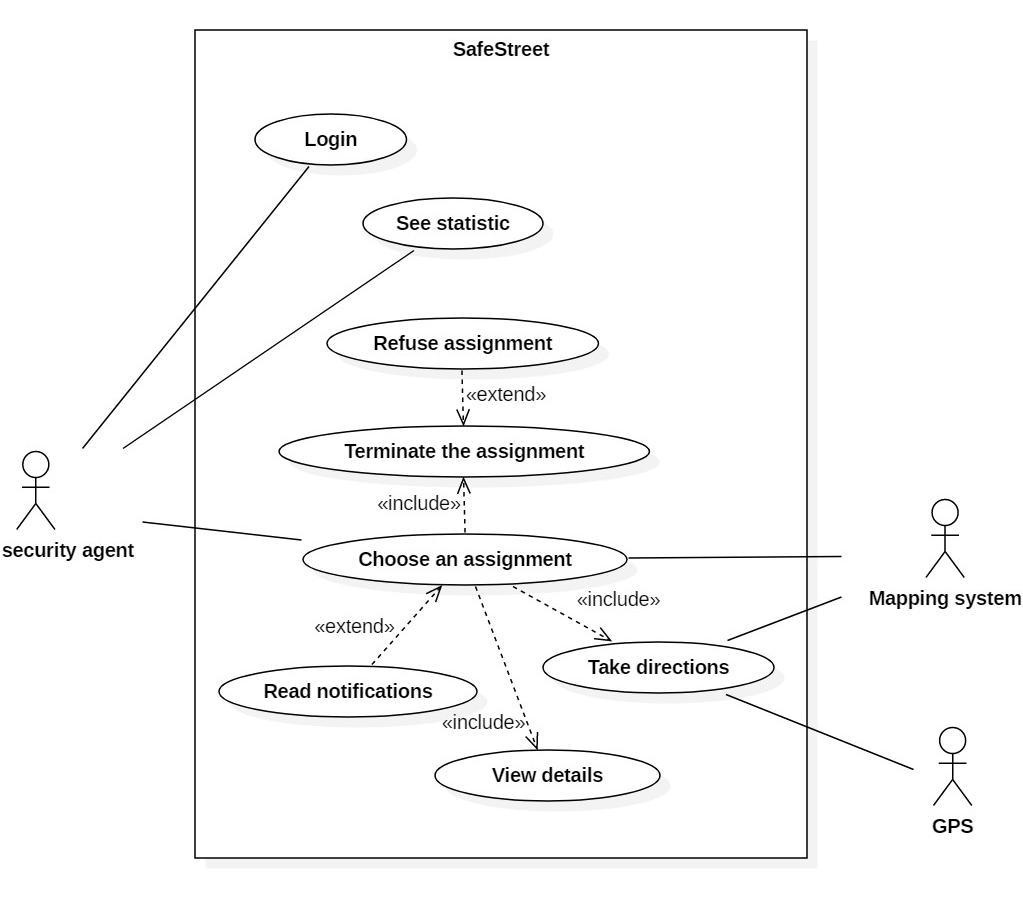
\includegraphics{Images/usecase_agent.png}
\caption{\label{fig:AUC}Authority Use Case }
\end{figure}
\begin{figure}[h]
\centering
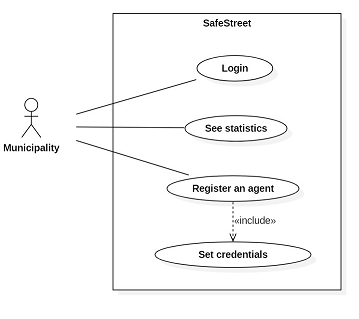
\includegraphics{Images/usecase_municipality.png}
\caption{\label{fig:MUC}Municipality Use Case }
\end{figure}
\begin{figure}[h]
\centering
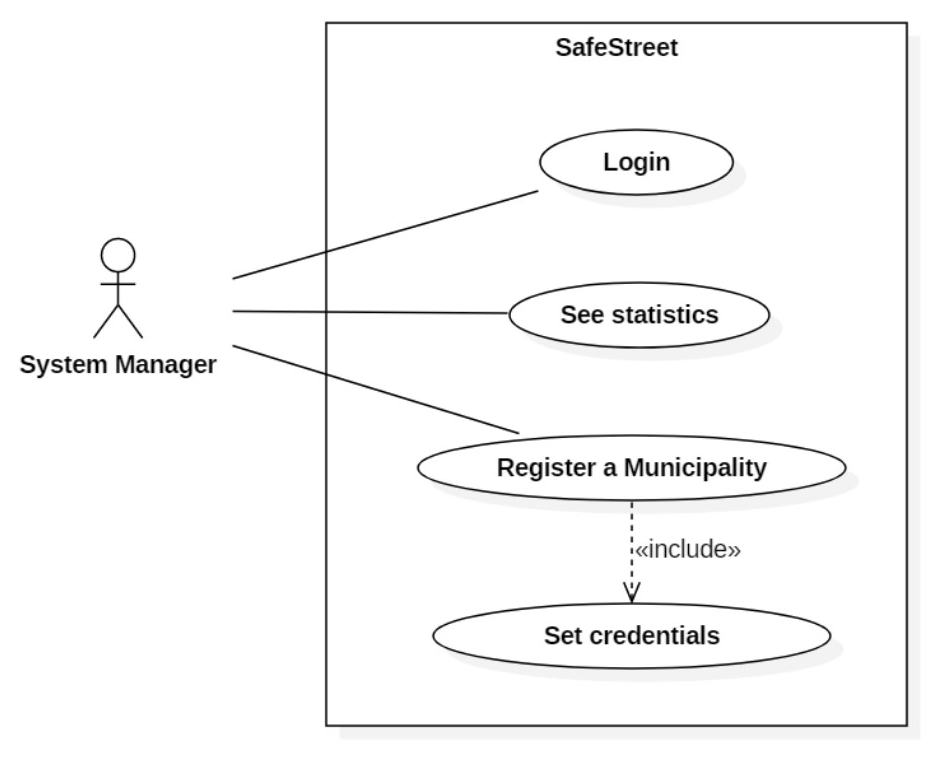
\includegraphics{Images/usecase_system_manager.png}
\caption{\label{fig:SMUC}System Manager Use Case }
\end{figure}
%.--------------------------------------------------------------------------------------------------------------------------------------------------------------
\subsubsection{Use Case Descriptions}
\begin{figure}[h]
\centering
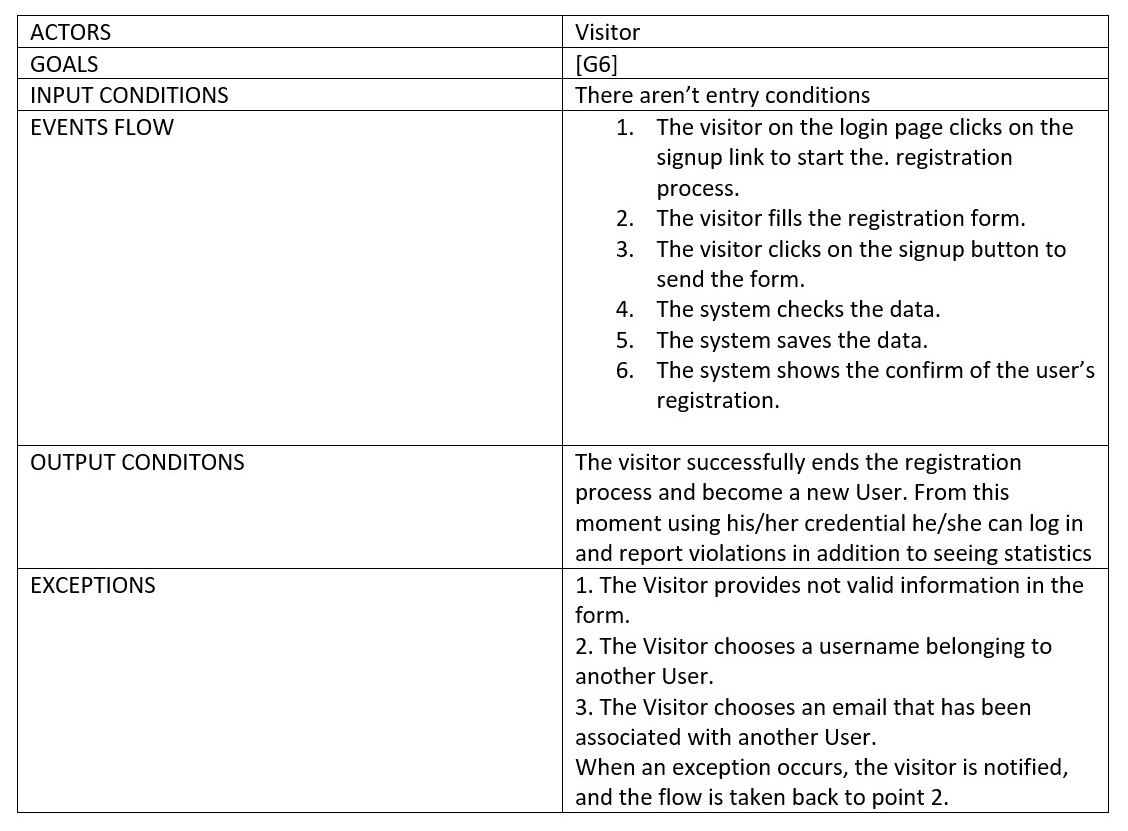
\includegraphics[width=\textwidth]{Images/visitor_use_case.png}
\caption{\label{fig:VUCD}Visitor Use Case Description}
\end{figure}
\begin{figure}[h]
\centering
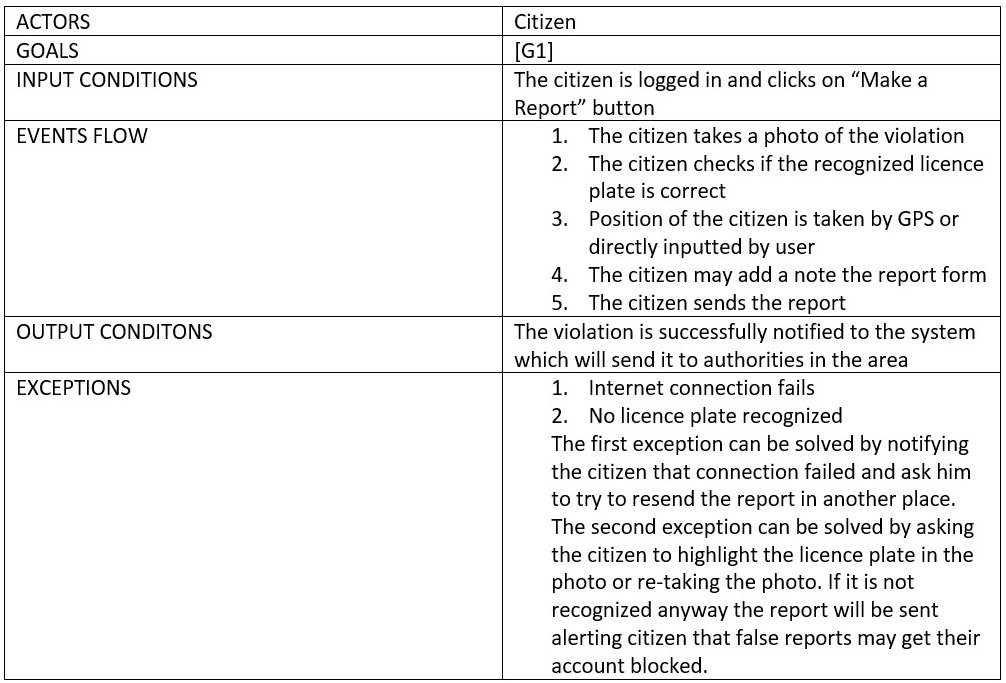
\includegraphics[width=\textwidth]{Images/citizen_use_case.png}
\caption{\label{fig:CUCD}Citizen Use Case Description }
\end{figure}
\begin{figure}[h]
\centering
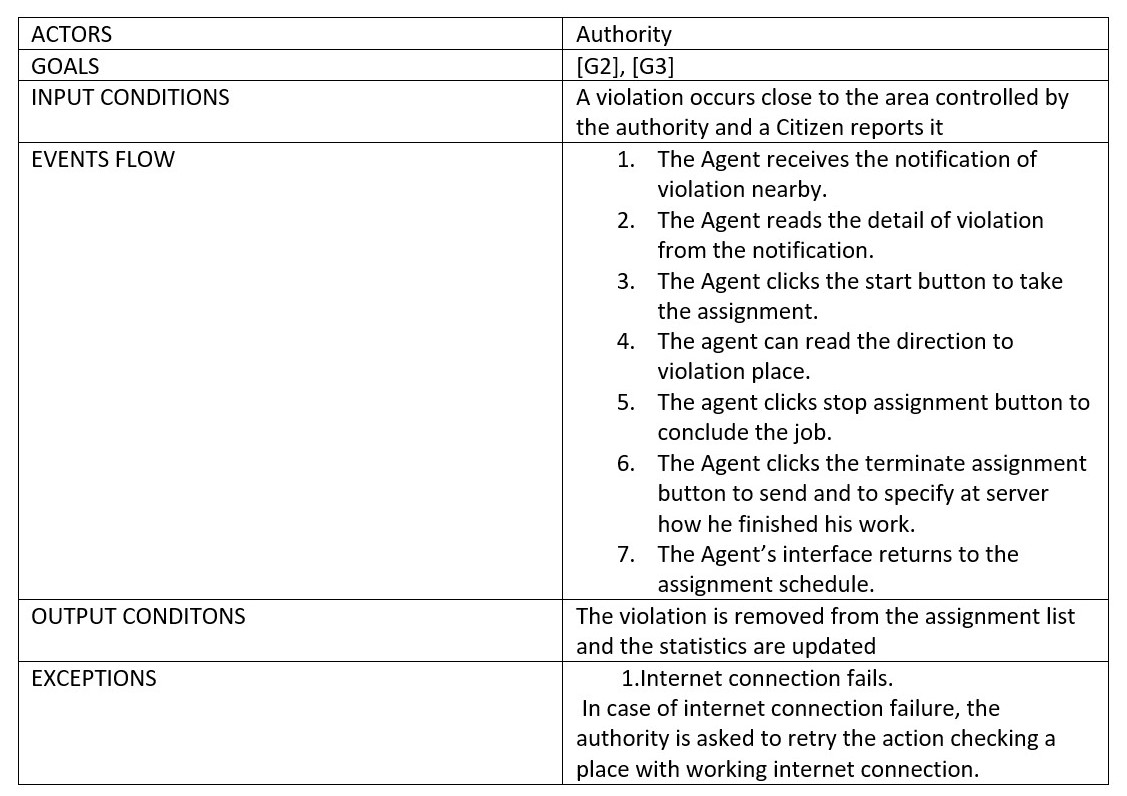
\includegraphics[width=\textwidth]{Images/authority_use_case.png}
\caption{\label{fig:AUCD}Authority Use Case Description 1}
\end{figure}
\begin{figure}[h]
\centering
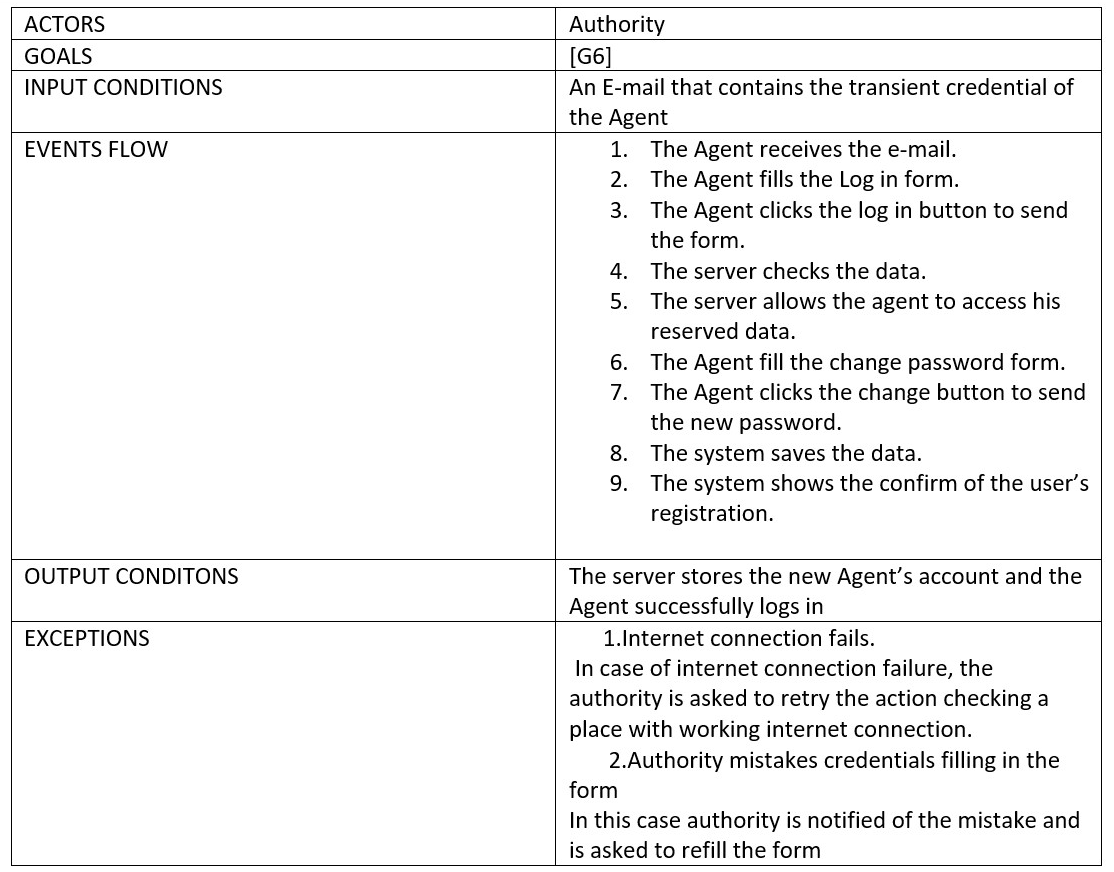
\includegraphics[width=\textwidth]{Images/authority_use_case2.png}
\caption{\label{fig:AUCD2}Authority Use Case Description 2}
\end{figure}
\begin{figure}[h]
\centering
\includegraphics[width=\textwidth]{Images/Municipality_use_case2.png}
\caption{\label{fig:MUCD}Municipality Use Case  Description 1}
\end{figure}
\begin{figure}[h]
\centering
\includegraphics[width=\textwidth]{Images/Municipality_use_case2.png}
\caption{\label{fig:MUCD2}Municipality Use Case  Description 2}
\end{figure}
\begin{figure}[h]
\centering
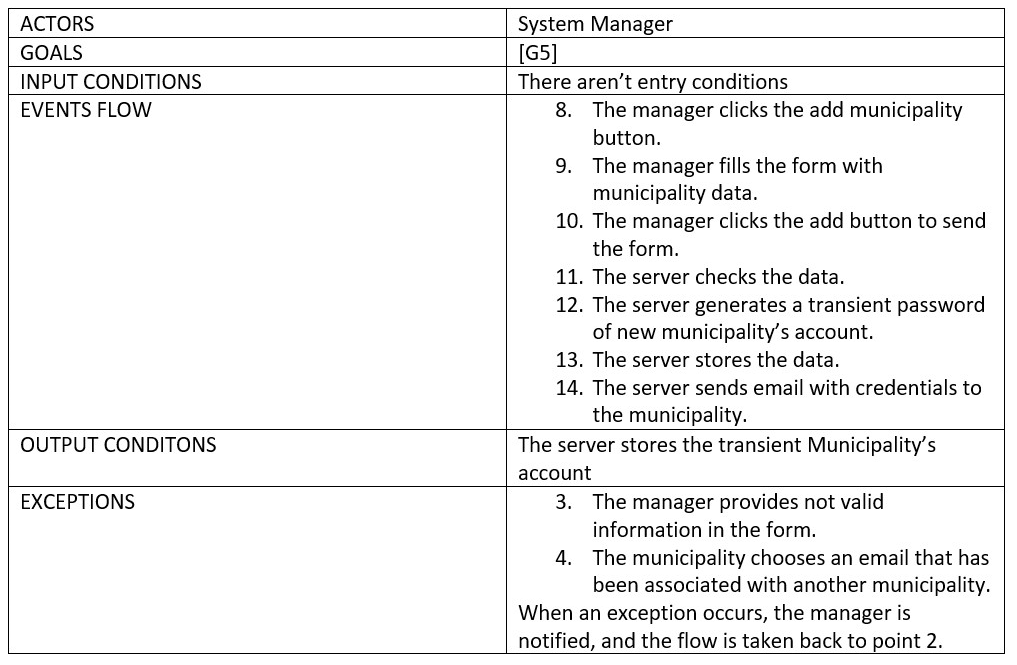
\includegraphics[width=\textwidth]{Images/system_manager_use_case.png}
\caption{\label{fig:SMUCD}System Manager Use Case  Description}
\end{figure}
\begin{figure}[h]
\centering
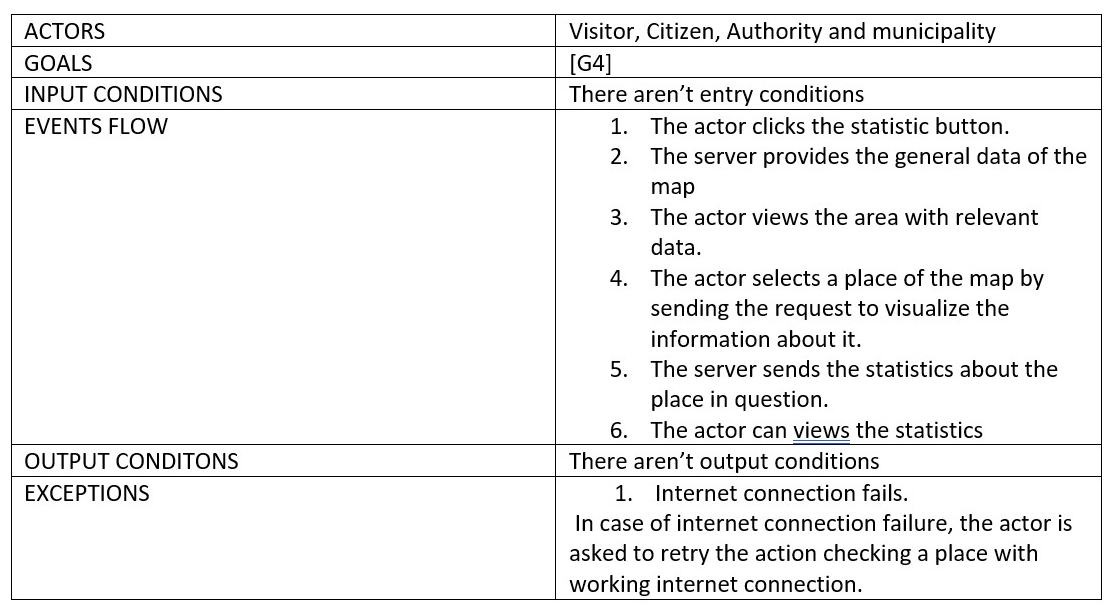
\includegraphics[width=\textwidth]{Images/common_use_case.png}
\caption{\label{fig:CUC}Common Use Case  Description 1} 
\end{figure}
\begin{figure}[h]
\centering
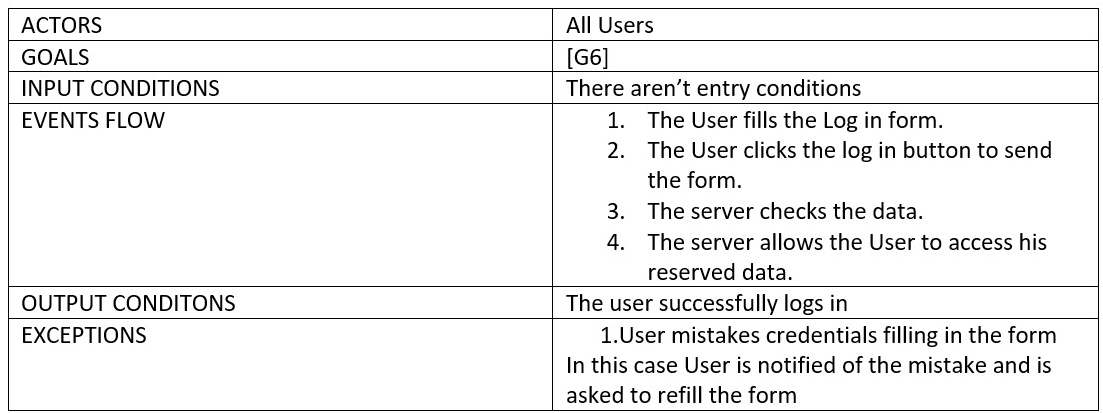
\includegraphics[width=\textwidth]{Images/common_use_case2.png}
\caption{\label{fig:CUC2}Common Use Case  Description 2}
\end{figure}
%.-------------------------------------------------------------------------------------------------------------------------------------------------------------
\subsubsection{Sequence  Diagrams}
\begin{figure}[h]
\centering
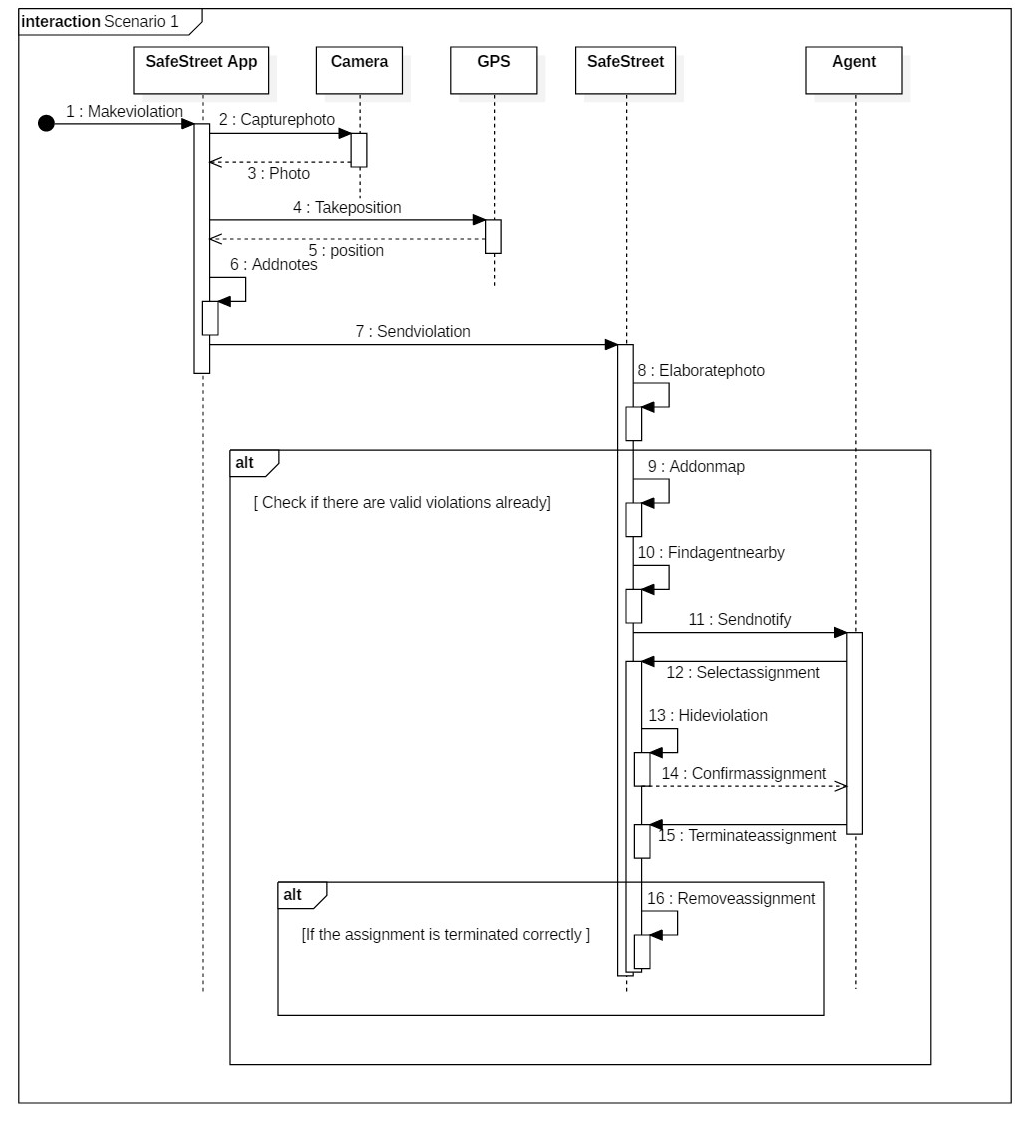
\includegraphics{Images/sequence_scenario1.png}
\caption{\label{fig:SDS1}Sequence Diagram Scenario 1}
\end{figure}
\begin{figure}[h]
\centering
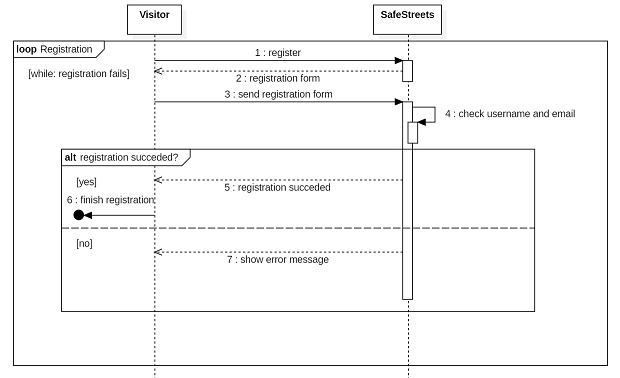
\includegraphics{Images/sequence_registration.png}
\caption{\label{fig:SR} Sequence Diagram Registration}
\end{figure}
\begin{figure}[h]
\centering
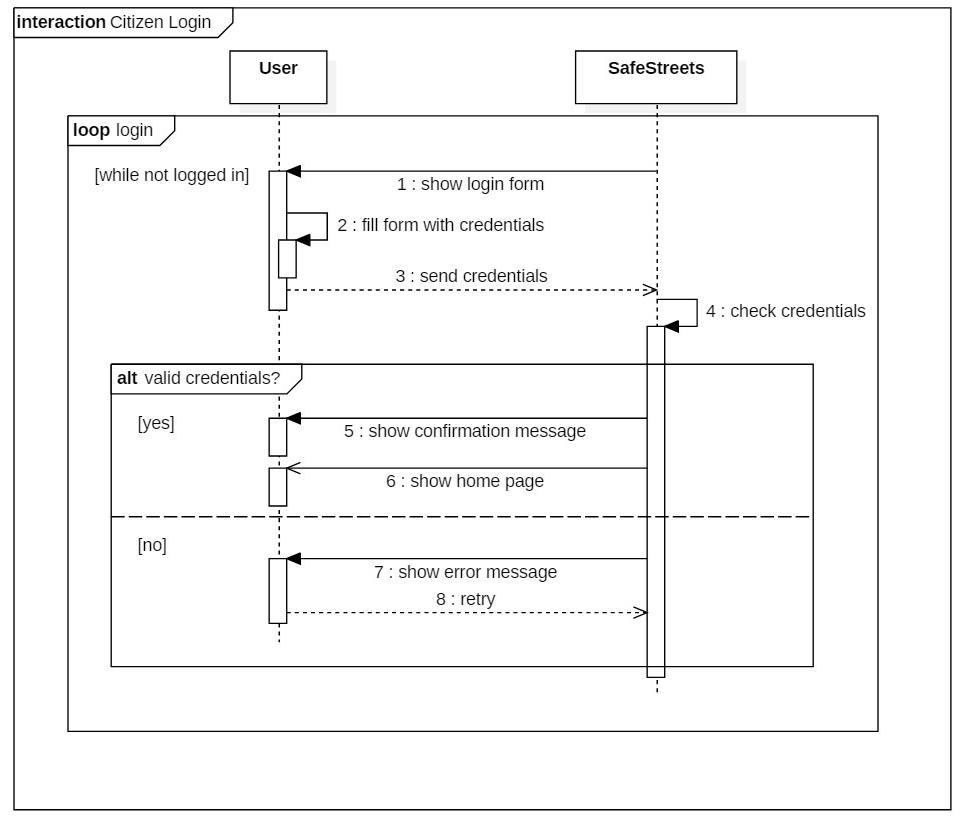
\includegraphics{Images/sequence_login.png}
\caption{\label{fig:SDL}Sequence Diagram Login}
\end{figure}
\begin{figure}[h]
\centering
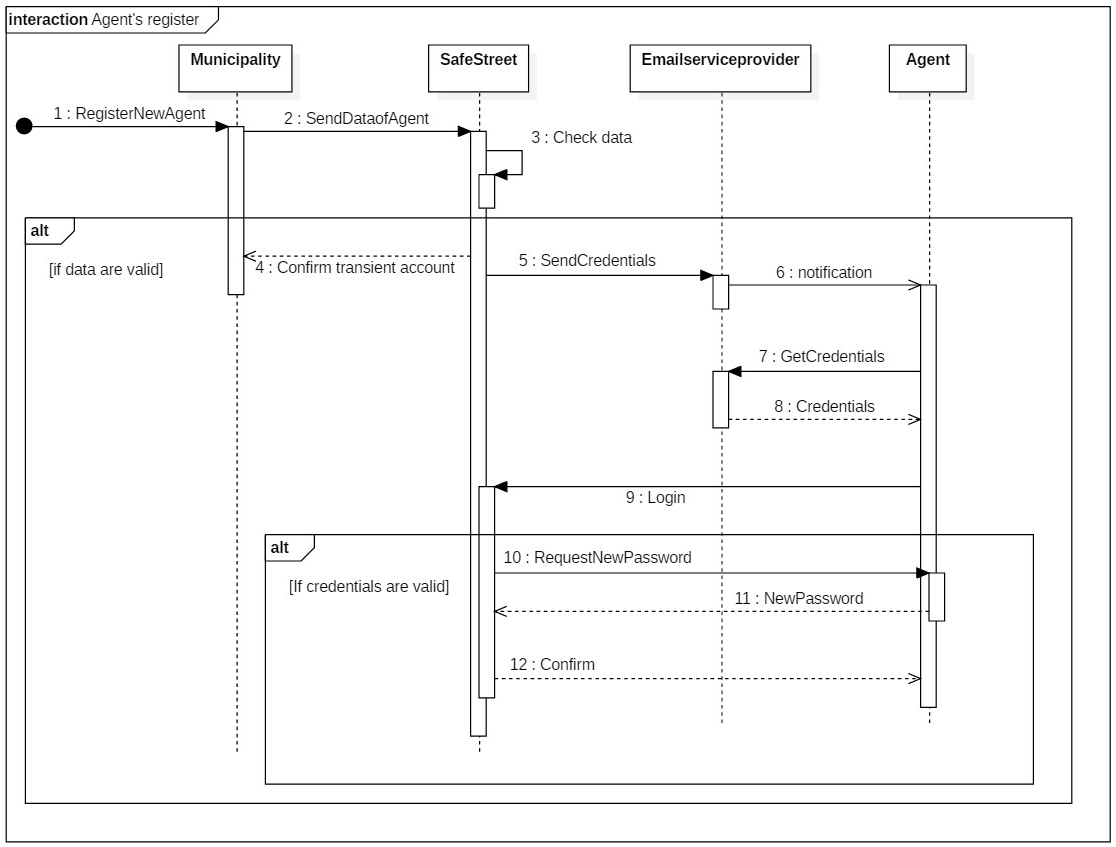
\includegraphics{Images/sequence_agent_register.png}
\caption{\label{fig:SDAR}Sequence Diagram Agent Registrtion} 
\end{figure}

%.-------------------------------------------------------------------------------------------------------------------------------------------------------------
\subsubsection{Mapping of Requirements and Domain Assumptions to their relative goal}
\begin{itemize}
\item G1) Notify authorities about traffic violations
\begin{itemize}
 \item R1) Authorities’ location must be known by the system when they are in service
 \item R2) When a Citizen makes a report the position is correctly added with the GPS when is available.
 \item R3) The right authorities are notified about violations.
 \item R10) When GPS is not available the user can input the position from a map.
 \item R11) Users to use the full service must be able to login providing the right credentials.
 \item D1) For each notification data and metadata provided by the system of the mobile phone are
correct.
 \item D3) GPS of authorities devices works correctly and gives the correct position every time.
 \item D4) Authorities if available correctly informs the system about their availability.
\end{itemize}
\item G2) Authorities must be able to take an available assignment
\begin{itemize}
 \item R1) Authorities’ location must be known by the system when they are in service.
 \item R3) The right authorities are notified about violations.
 \item R11) Users to use the full service must be able to login providing the right credentials.
 \item D3) GPS of authorities devices works correctly and gives the correct position every time.
 \item D4) Authorities if available correctly informs the system about their availability.
 \item D6) System Manager, Municipality and authorities respects their duty of care.
\end{itemize}
\item G3) Allow authorities to report a finished assignment
\begin{itemize}
 \item R4) Authority must be able to provide the system how the assignment finished: resolved and the
type of violation, no intervention needed when arrived, false report.
 \item R11) Users to use the full service must be able to login providing the right credentials.
 \item D6) System Manager, Municipality and authorities respects their duty of care
 \item D8) Information provided by authority are correct and no false report is ignored.
\end{itemize}
\item G4) Allow all actors to visualize updated statistics
\begin{itemize}
\item R5) The system must make Statistics available when asked.
\item R6) Statistics are always updated when an event happens.
 \item D8) Information provided by authority are correct and no false report is ignored.
\end{itemize}
\item G5) Allow the system manager to register Municipality to the service
\begin{itemize}
\item R7) For registering a Municipality his/hers data must be provided to a System manager who will add those data to the service to sign up him/her.
\item R9) When the creation of an account is successful the system must notify the Visitor sending an email to the address provided in the sign up process.
 \item R11) Users to use the full service must be able to login providing the right credentials.
\item D6) System Manager, Municipality and authorities respects their duty of care
\end{itemize}
\item G6) Allow a Visitor to join the system registering him/herself to ensure reliability of the information provided by him/her
\begin{itemize}
\item R8) A visitor must be able to begin sign up process in the SafeStreets App filling a form with his
data.
\item R9) When the creation of an account is successful the system must notify the Visitor sending an
email to the address provided in the sign up process.
 \item R11) Users to use the full service must be able to login providing the right credentials.
 \item R15) Each Username is unique
\end{itemize}
\item G7) Store information about violations provided by users:
\begin{itemize}
 \item R2) When a Citizen makes a report the position is correctly added with the GPS when is available.
 \item R4) Authority must be able to provide the system how the assignment finished: resolved and the
type of violation, no intervention needed when arrived, false report.
 \item R10) When GPS is not available the user can input the position from a map.
 \item R12) The camera of the mobile phone must be accessible to take photos of violations.
 \item R14) The User must be able to select the licence plate between the ones in output from the Licence
Plate Recognition algorithm.
 \item D8) Information provided by authority are correct and no false report is ignored.

\end{itemize}
\item G8) Identify potentially unsafe areas:
\begin{itemize}
\item R4) Authority must be able to provide the system how the assignment finished: resolved and the
type of violation, no intervention needed when arrived, false report.
\item R6) Statistics are always updated when an event happens.
\item D1) For each notification data and metadata provided by the system of the mobile phone are
correct
\item D8) Information provided by authority are correct and no false report is ignored.

\end{itemize}
\item G9) Allow municipality to register Authorities to the service
\begin{itemize}
\item R9) When the creation of an account is successful the system must notify the Visitor sending an
email to the address provided in the sign up process.
\item D6) System Manager, Municipality and authorities respects their duty of care
\item D7) When an authority is sent an email to register this will surely be received
\item D9) The Agent and municipality must be able to communicate
\item D10) Information of authority which is being registered are known by municipality
\end{itemize}
\item G10) Help the Municipality to make decision 
\begin{itemize}
\item R6) Statistics are always updated when an event happens.
\item R11) Users to use the full service must be able to login providing the right credentials.
\item R13) Suggestions must be available when municipalities request them.
\item D11) The data of external database are always available.
\end{itemize}
\end{itemize}

%.-------------------------------------------------------------------------------------------------------------------------------------------------------------
\subsection{Performance Requirements}
The system should be able to respond to a possibly great number of simultaneous requests. Based on 
data about Milan, there are over 100.000 parking violations a day, so the system should be able to keep 
track of at least 10 times that number of notifications a day. In some special cases, like public transport 
strikes, the number of violations could increase sensibly and the server could have to manage a lot of 
requests.

%.-------------------------------------------------------------------------------------------------------------------------------------------------------------
\subsection{Design Constraints}
%.-------------------------------------------------------------------------------------------------------------------------------------------------------------
\subsubsection{Standards compliance }
SafeStreets aims to become the smartest and quickest way to report violations in Italy. 
Nowadays, citizens who want to send a report can contact the authorities by calling an emergency number, 
but this can take a lot of time. Moreover, during critical events, phone lines could be unavailable. 
You can also use police website, but its interface is not user-friendly. In any case, you can’t send any 
evidence of the violation to the authorities. Anyway, the idea of our service is not unique: there are already 
similar services in other countries, like in India where there is “Public Eye. OFFICIAL BTP APP”.
%.-------------------------------------------------------------------------------------------------------------------------------------------------------------
\subsubsection{Hardware limitations}
\begin{itemize}
\item Mobile App
\begin{itemize}
\item Android smartphone
\item 2G/3G/4G connection
\item GPS
\end{itemize}
\item Web App
\begin{itemize}
\item Modern browser able to retrieve user's location
\end{itemize}
\end{itemize}
%.-------------------------------------------------------------------------------------------------------------------------------------------------------------
\subsection{Software System Attributes}
%.-------------------------------------------------------------------------------------------------------------------------------------------------------------
\subsubsection{Availability}
The system should be available 99,99\% of time. Considering only one State, there will be a time range 
in which notifications are considerably reduced (the night-time when citizen will less likely report 
a violation) and so reliability constraint for night-time could be reduced up to 99\% reducing also some 
resources allocated to the system.
%.-------------------------------------------------------------------------------------------------------------------------------------------------------------
\subsubsection{Reliability}
There are no strict costraints of Reliability if Availability costraints are respected
%.-------------------------------------------------------------------------------------------------------------------------------------------------------------
\subsubsection{Security}

Users credentials will be stored. Security of the data and of the communications user-system is a primary concern.

%.-------------------------------------------------------------------------------------------------------------------------------------------------------------
\subsubsection {Maintainability}
The system must be developed in a modular way so that new feature can be added.
Using a modular approach it is also possible to test the functionality of the single parts making it simpler to maintain.
Documentation must be also always updated in case of modifications of the system to always keep documentation aligned to the system.
%.-------------------------------------------------------------------------------------------------------------------------------------------------------------
\subsubsection{Scalability}
This system is designed to be optimized in Italy. It is possible to expand it later by choosing a more suitable
algorithm to recognize licence plates and by dividing computation of different states on different servers, so that reliability analysis made for Italy are still true for every single state. Information about boundaries
of states should be replicated in both states making the transition from one server to the other smoother.
%.-------------------------------------------------------------------------------------------------------------------------------------------------------------
\subsubsection{Accuracy}
Accuracy of the position of authorities and violations has to be the best possible. All the sensors used must provide positions' data with an error lower than 20 meters. We can consider a larger bound of accuracy because authorities work on a given area so from a well taken photo, they should be able to recognize the place of the violation even if the position given by the GPS is not too accurate.












%------------------------------------------------------------------------------------------------------------------------------------------------
\clearpage
{\color{Blue}{\section{Development Choices}}}
\label{sect:Development Choices}
%.-------------------------------------------------------------------------------------------------------------------------------------------------------------
\subsection{Adopted Programming Languages}
%.-------------------------------------------------------------------------------------------------------------------------------------------------------------
\subsubsection{Back End}
For the developing of the back-end of the we used Java.
We choose java for it being cross-platform, so the possibility of running the code on different machines. Even though the back-end prototype is developed in a single machine this choice allows with some modification to deploy different components on different machine and use functionality like Java Remote Method Invocation to communicate. The choice is also driven by the variety of functionality JEE has. JEE has components for database access but also for the creation of Http Servers.
Another advantage of using Java is being Object Oriented and allowing Polymorphism and Inheritance allowing the user to create a structure for a general Object and expanding it in different forms. This allowed a really fast developing of the Response Objects which the server returns to the client.
Other advantages in the development are the usage of annotations to enforce properties to functions (I.e.@Override) and last but not least automatic garbage collection.
Garbage collection is an advantage for developing an application since it removes part of the controls the developer must perform it also adds a considerable drawback of slowing down the application if object are created and than discarded continuously.
To remove part of this overhead the use of Object Pooling techique for the most resource consuming Objects is applied, in the project we used an Object Pool for Database Connections. 

\subsubsection{Front End: Web Application}
To develop the front end we used javascript with jquery and leaflet.
Jquery allows to write more readable code than javascript and simplifies the developement, also caching mechanism of browsers may 
allow users to load it from memory if it is already cached. A disadvantage is the difficulty to develop with different components and pages and in most cases the code written is only usable in one or few pages. Being the web applicaiton developed rather small it was possible to develop it without using complex frameworks.
Leaflet is a lightweight javascript map library. It provides the functionalities required by the software with a quick loading time and an easy inclusion in the application.

\subsubsection{Front End: Why no Mobile Application in the prototype?}
We have chosen not to implement the mobile application because its only use was to communicate with the server and show data to the users. This functionalities can be found in the web interface; in fact, in order to test and develop the prototype, we have chosen only the web interface to uniform the front end structure. In ths way, we can also reuse components employed in interactions through the users

%.-------------------------------------------------------------------------------------------------------------------------------------------------------------
\subsection{Software used}
%.-------------------------------------------------------------------------------------------------------------------------------------------------------------
\subsubsection{Back End}
The Back End developement was carried on using different softwares:
\begin{itemize}
\item Eclipse IDE for Java EE Developers :  This IDE provides a rich environment to develop applications in Java. Eclipse has components for managing projects and the dependencies of the project . The IDE also supports JUnit Test Suite and allows to do Coverage testing.
It also allows to work with git inside it to manage versioning of the project.
We used it also for developing of the web App since it allows editing also of javascript ,html and css files.
\item MySQL : MySQL is a relational DBMS easy to set-up, to export and import using MySQL workbench GUI.
				The GUI allows also simple table creation , table value modifications, stored procedure creation and trigger creation
				It is also easy to connect from the Java Code .
\item Apache Tomcat : Tomcat  is an open source implementation of the Java Servlet. This software is used to deploy the Back End.
						Using Eclipse IDE for the developement after downloading Tomcat the setup is really fast and easy.
\end{itemize}
\subsubsection{Front End}
The front end was developed using Eclipse IDE (described before).


%.-------------------------------------------------------------------------------------------------------------------------------------------------------------
\subsection{Adopeted API}
%.-------------------------------------------------------------------------------------------------------------------------------------------------------------
\subsubsection{Back End}
In the developement of the Back End we used the API provided by Mysql server to connect to the database , the API of tomcat servlets to develop and deploy servlets and the Java Mail Api to send emails to the users.
\subsubsection{FrontEnd}
FIn the developement of the Front End we used the API provided by openStreetMaps in the web Application to get the map shown with leaflet and the geolocation API provided by the browser to get the user position. We also used APIs provided by OpenALPR in order to recognize licence plate thought Optical Character Recognition technology.




%------------------------------------------------------------------------------------------------------------------------------------------------
\clearpage
{\color{Blue}{\section{Structure of the source code}}}
\label{sect:Structure of the source code}
%.-------------------------------------------------------------------------------------------------------------------------------------------------------------
\subsection{Back-end}
\subsubsection{Package diagram}
The Java code has a Javadoc which can be accesssed in \href{https://github.com/pm390/MaldiniPaone/tree/master/Implementation\&Testing/SafeStreets/doc}{our github repository} 
Here we present the overall structure of the project at different levels.
\begin{figure}[h]
\centering
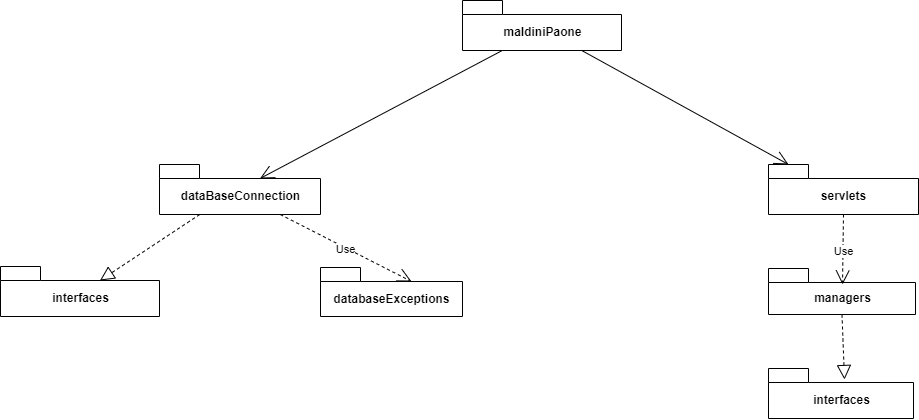
\includegraphics[width=\textwidth]{Images/packageDiagram.png}
\caption{\label{fig:pK} Package diagram of the main packages}
\end{figure}
In this diagram a basic view of the code structure is seen. The source can be divided in mainly two sub-parts. The first part concerning the connection to the database which is handled by the classes in the databaseConnection package and a second part
which communicates with client devices which is handled by the Servlets implemented in the servlet package.
The database Connection package has two sub packages one to define the interfaces it exposes to the other classes, the other with the Exception Classes which can be thrown by the classes in the package.
The servlets package classes communicates with the managers in the managers packkage which provides interfaces to allow access to the needed functionalities.
In this diagram the utilities package and it's sub packages are not shown for the sake of clarity. 
This package contains useful objects, beans and constants which are used through the whole developement.
\clearpage
\subsubsection{ Database Connection}
\begin{figure}[h]
\centering
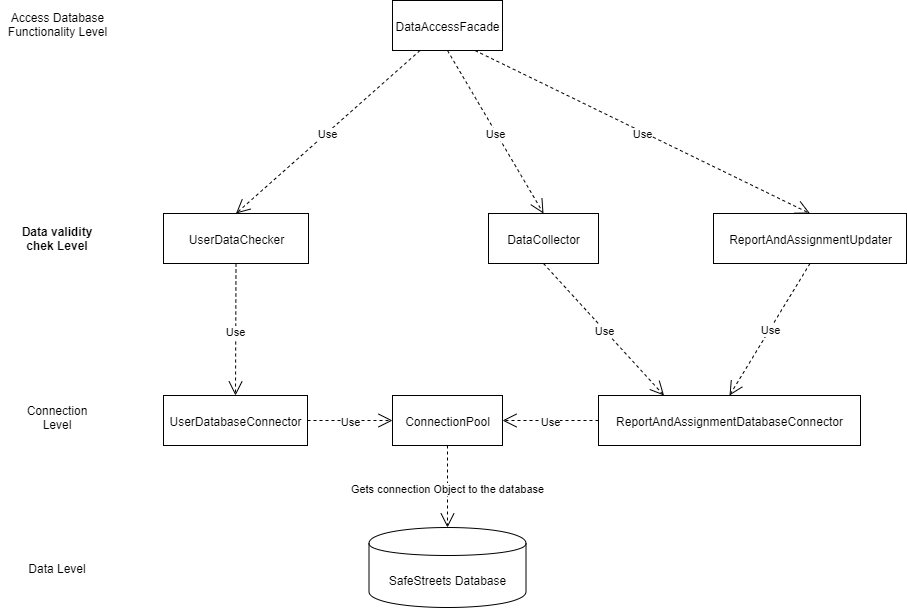
\includegraphics[width=\textwidth]{Images/databaseConnection.png}
\caption{\label{fig:pK} databaseConnection classes}
\end{figure}
This diagram shows the Classes in the databaseConnection package the database is also shown to present which component instantiates connection with it. A clear separation of concerns is shown between the different classes:
\begin{itemize}
\item Connection Level : classes in this level have 2 main functions the instantiation of connection which is done by the ConnectionPool and using the instatiated connections to get data ,save data, update data from the database.
The latter function is implemented in two separated classes to divide the class managing information concerning the user accounts and the one managing information concerning reports and assignments.
Implements the functionalities.
\item Data validity check Level: classes in this level checks that input values for accessing the database are correct. This layer protects the possible accesses to the database with invalid values avoiding the instantiation of useless connection which may slow down the server. This level throws the appropriate exceptions if the database connection couldn't be instantiated on the lower level or if the parameters are invalid.
Controls access to the functionalities.
\item Access Database Functionality Level : this level contains a class DataAccessFacade as the name says it is a facade and so it presents to the other packages the functionalities that the database conneciton package provides. This layer contains almost only call to functions provided by the beneath level to allow a clear separation of the functionalities of the package.
Allows access to the functionalities.
\end{itemize}
\clearpage
\subsubsection{Servlets}
\begin{figure}[h]
\centering
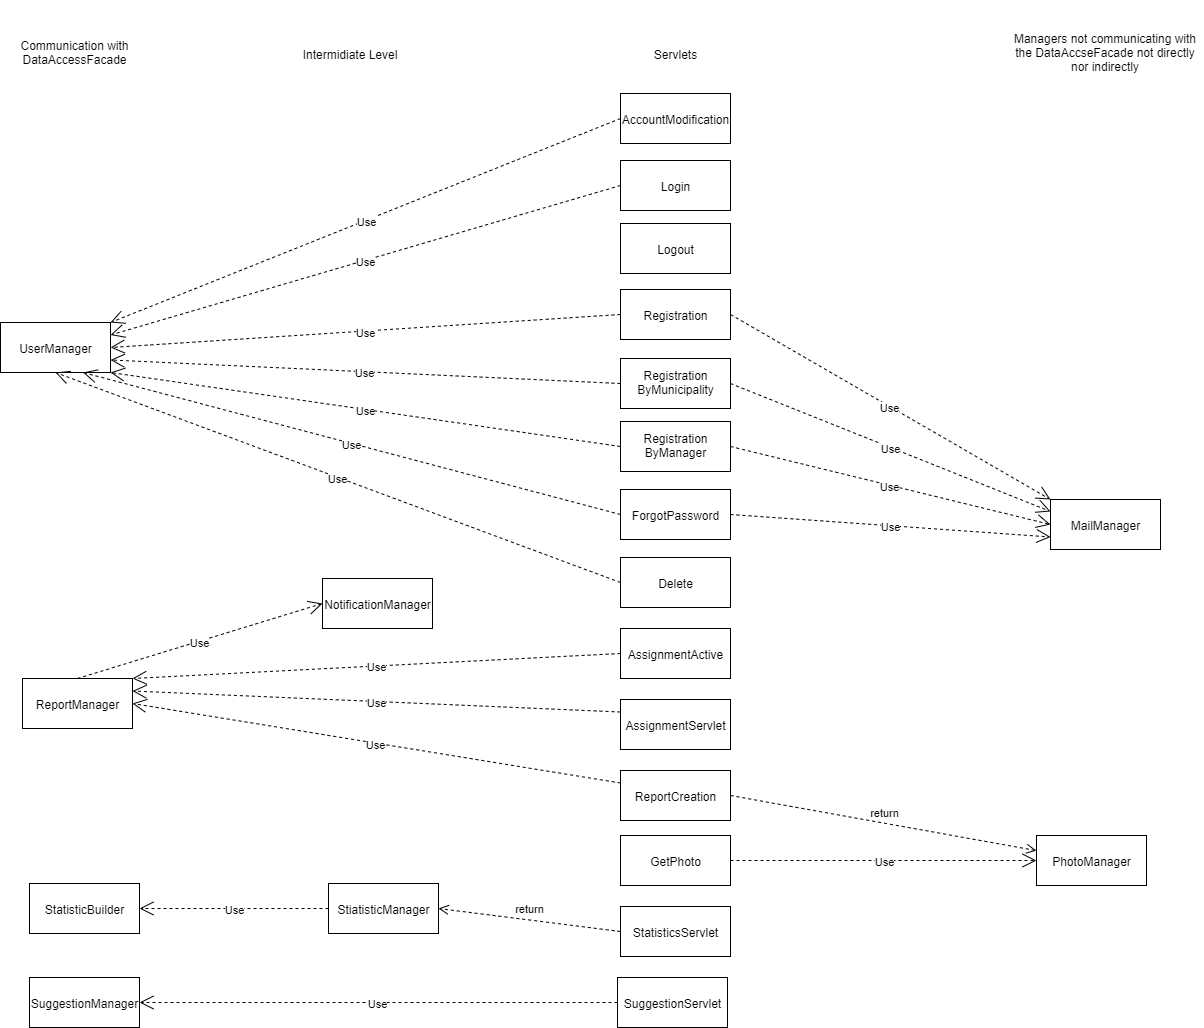
\includegraphics[width=\textwidth]{Images/Servlets.png}
\end{figure}
The Servlet package's classes are shown in the above diagram.
The functionalities provided by the servlets to the end users are provided to the servlets by managers in the package. 
The managers  on the left part communicates with the DataAccess facade to retrieve, save or modify data on the database 
The Intermediate level shown Contains classes which communicates indirectly with the database because informations used by it comes from communications with the database. The servlets provides functionalities of the service to the clients of the web application and of the mobile application.
On the right part of the image 2 managers are shown. Those managers doesn't communicate directly with the database and allows the system to save photos and to send mails to the clients.
\clearpage
\subsection{Front End }
\subsubsection{Web App}
The web application is composed of an html file , a css file developed by us , css files of leaflet to present the map , external javascript imported libraries(jquery, leaflet and openAlpr) and different javascript source files.
The html file contains the single page application which allows municipalities and managers to access their functionalities.
The javascript source files are basicFunctionalities.js and ourMap.js, the first source adds to the page the dinamic behaviour of buttons and avoids synchronous requests to the server using ajax get and post requests, the second source handles the creation of the map and the binding of events to update the map and defines the  behaviour when the user clicks on markers on the map, the other javascript files are used to set up the functionalities of open alpr and use them to recognize license plates in a photo.



%------------------------------------------------------------------------------------------------------------------------------------------------
\clearpage
{\color{Blue}{\section{Testing}}}
\label{sect:Testing}
%.-------------------------------------------------------------------------------------------------------------------------------------------------------------

\subsection{Back end Testing}
For the Backend testing we created two jUnit test classes to test functionalities of user creation and creation and modification of reports and assignments. Here we first created some random Location objects and we checked that location with invalid coordinates can't be created using a coverage test to see if the test case actually tries to create them and the correct exception is cached. After this some users of every type are created. Every time a new user is created we try to create a second copy and check if that is not possible.
After creating users the reports are created using a username of the citizens created.
Later we make authorities accept the assignments created when adding the repots , than we make them terminate them.
Every time we update the state of an assignment we try to re-do the action to test if invalid modifications are not possible and are correctly handled.
For lack of time we didn't create actual test cases for functionalities outside the database connection package. 
For controlling functionalities we used console logging to try out functionalities and debug the system.
We tried different inputs and invalid inputs checking if the outputs are correct and if the error messages are correctly shown to the user.
For a final test we gathered a little group of people and we made them test the system on our computer giving them instructions to use the system.
If we had more time we would have created a full test suite containing also tests for servlets package instead of using only log functions. 
\subsection{Front End Testing}
For front end testing we covered the functionalities we wanted to offer to clients on the target devices to see if the interaction were correctly implemented. We controlled also that all the possible error messages were displayed to the user.
We were also helped by the group of people we gathered who provided us useful feedbacks for improving the user experience for later release. With more time we would have done a rework on the user interface to improve the experience of using our system.
%----------------------------------------------------------------------------------------------------------------------------------------------------------------------------------------------------------------------------------------------

%------------------------------------------------------------------------------------------------------------------------------------------------


\clearpage
{\color{Blue}{\section{Installation Instructions}}}
\label{sect:Installation Instructions}
%.-------------------------------------------------------------------------------------------------------------------------------------------------------------
\subsection{Install Java}
If you already have the latest version of java sdk skip this step.
Visit the \href{https://www.oracle.com/technetwork/java/javase/downloads/jdk13-downloads-5672538.html}{jdk installation page}.
Accept license agreement and install the version suitable for your operating system.
If you downloaded the executable execute it if you downloaded the zip version unzip it in a new directory called JAVA which you should place in the programs folder of your pc. 
\begin{figure}[h]
\centering
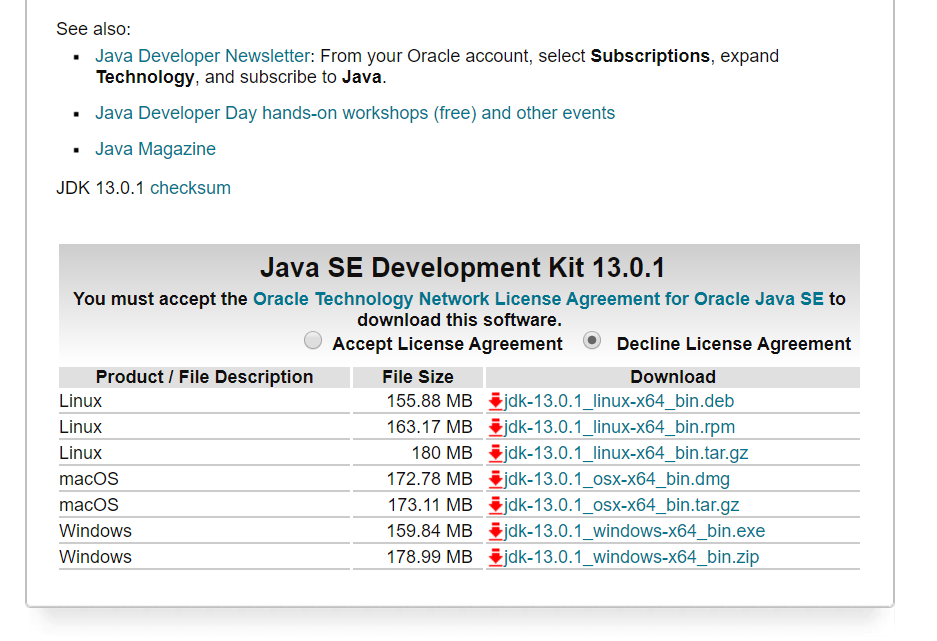
\includegraphics[width=\textwidth]{Images/javaVersionchoice.png}
\end{figure} 
\clearpage

\subsection{Set Up Java}

Set the environment variable JAVA\_HOME to the directory where you installed the jdk.
Normally the installation path will look like "C:\textbackslash Program-Files\textbackslash Java \textbackslash jdk-13.0.1" where jdk-13.0.1 could be different if you downloaded a more recent version. To set up environmente variable in windows search in the search bar of the pc "env" a choice with 
"Edit the system environment variables" or in italian " modifica le variabili di ambiente relative al sistema " should appear  
click it than click environment variable at the bottom right of the menu which appears. A new window should appear, check if the variable JAVA\_HOME is available in the list at the top, if it isn't  press add otherwise choose it and press modify. In the opened window insert as variable name JAVA\_HOME and as value the path of your jdk. After confirmation you can close all.

\begin{figure}[h]
\centering
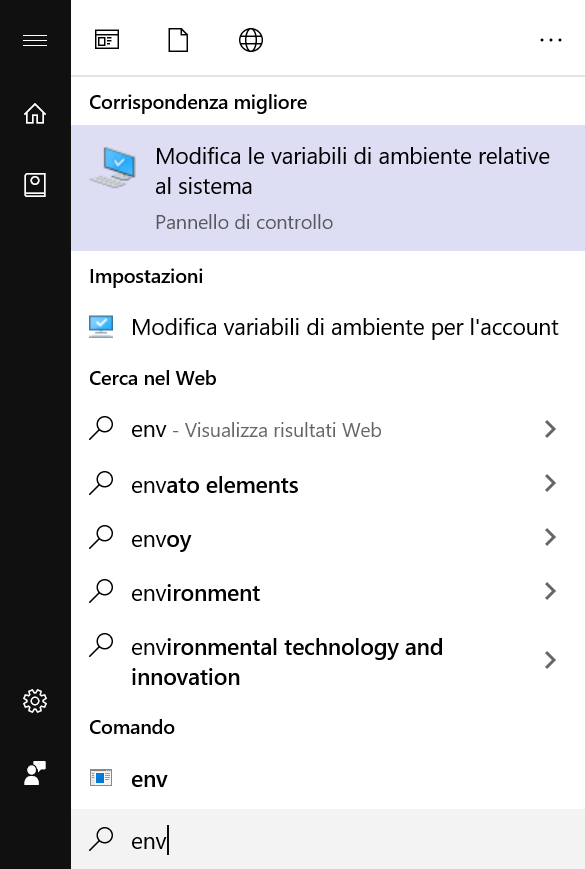
\includegraphics{Images/environment variable.png}
\end{figure} 

\begin{figure}[h]
\centering
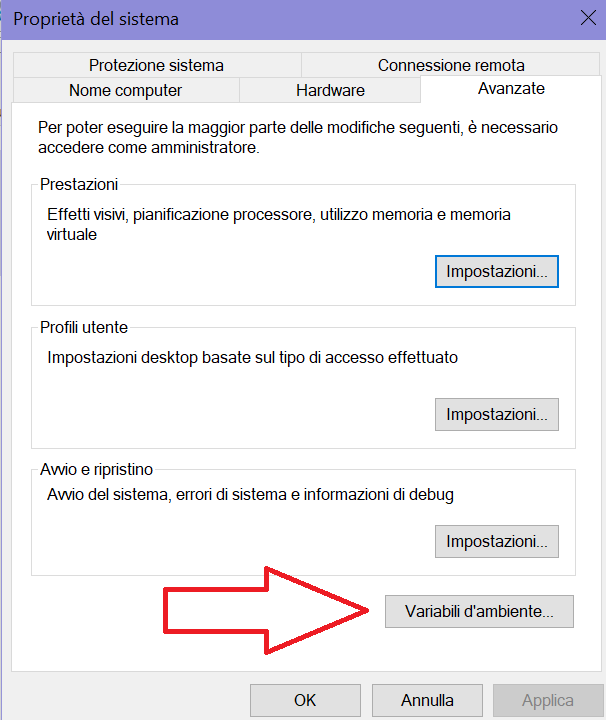
\includegraphics{Images/env.png}
\end{figure} 
\begin{figure}[h]
\centering
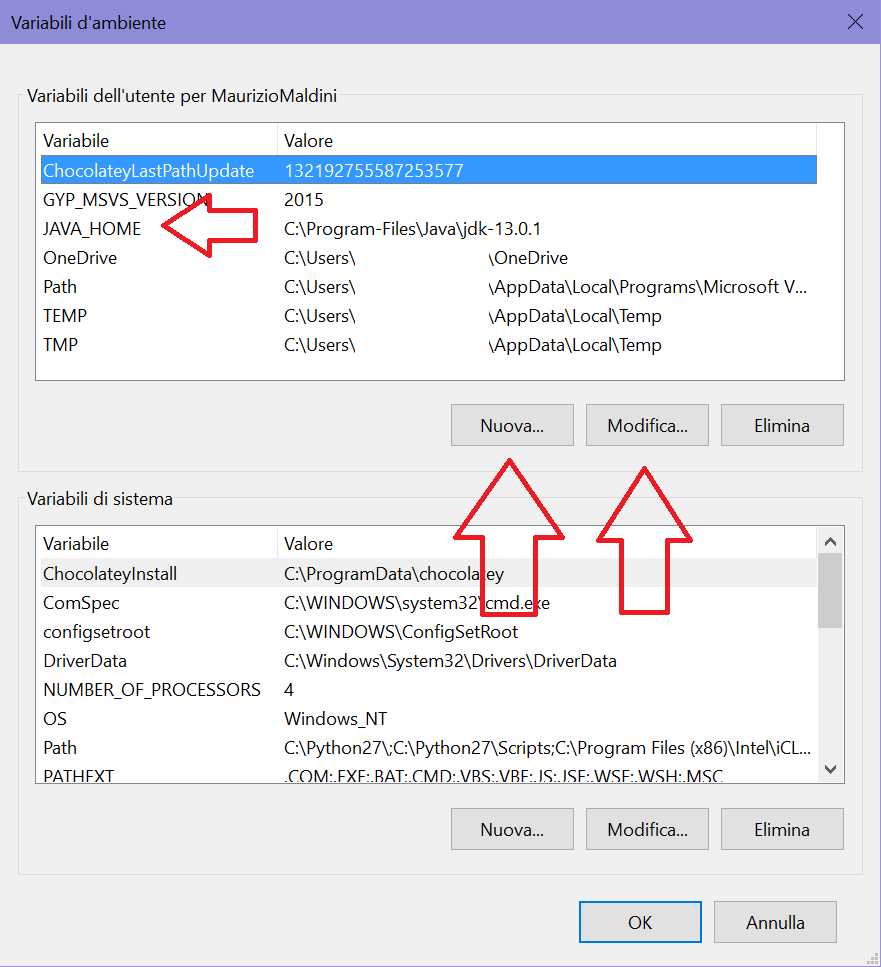
\includegraphics{Images/environment.png}
\caption{\label{fig:myi} Here you can see where java home should be visible if not available add it or update if it is outdated}
\end{figure} 

\begin{figure}[h]
\centering
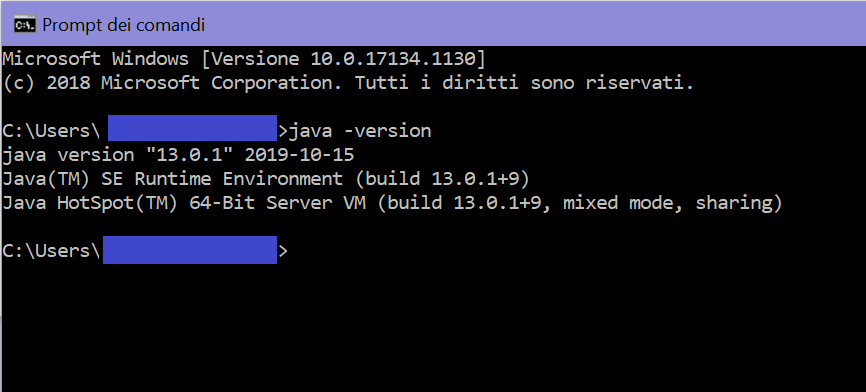
\includegraphics[width=\textwidth]{Images/javaInstallationCheck.png}
\caption{\label{fig:myi} Now go to the console (for windows in the search bar search "cmd" and open command prompt) wirte the commande java -version
you should get and output similar to this image.If you don't get a similar message check if the variable JAVA\_HOME is set correctly. If you get a different version from the one you installed check if you have other oracle products installation and check if they are not interfering with the environment.}
\end{figure} 



\clearpage
\subsection{Download Tomcat}
Visit the \href{https://tomcat.apache.org/download-90.cgi}{tomcat download page}.
Download the correct version of the binary distribution for your os. For a lightweight deployment we suggest the zip version.
Once downloaded unzip the folder. Open the folder and open the folder bin inside it, in this folder than execute the startup.bat for windows or startup.sh for linux. If java installation worked correctly and java home is set correctly you should get a screen like this one.
if you got this screen run the shutdown.bat or shutdown.sh to stop the server. If a console flashes in and disappear immediately there is an error in the java home variable.
\begin{figure}[h]
\centering
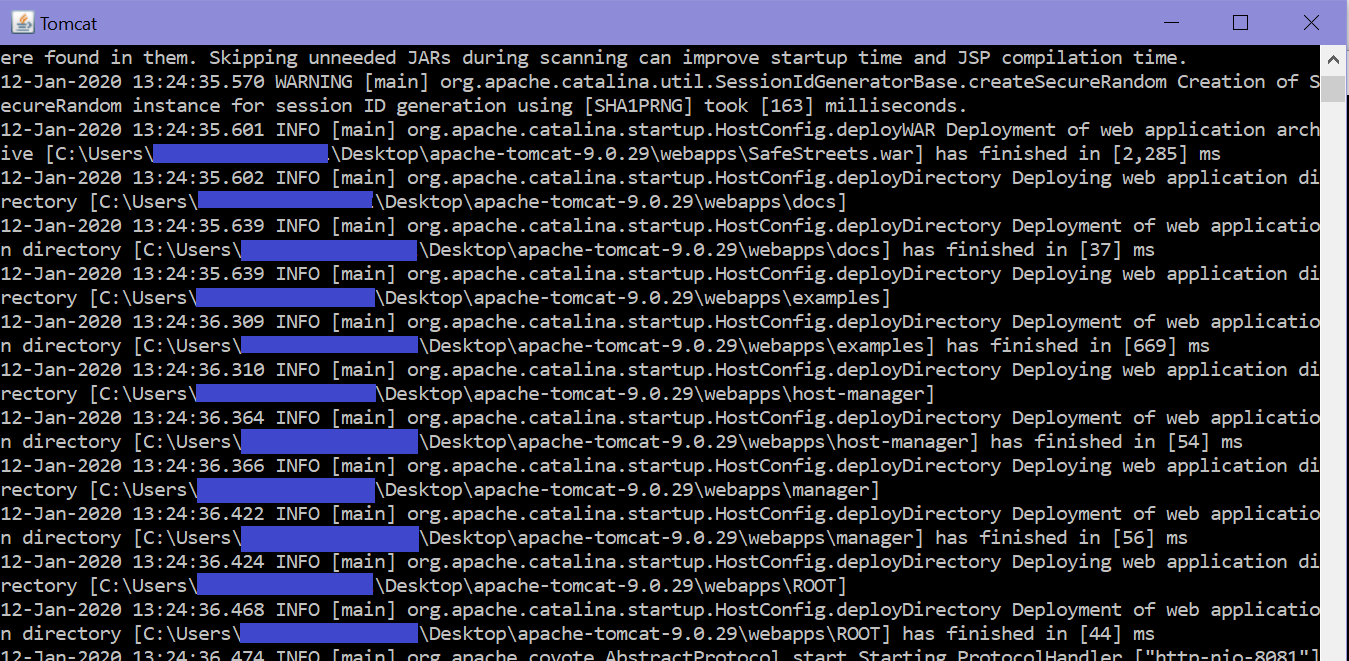
\includegraphics[width=\textwidth]{Images/tomcatStartup.png}
\end{figure} 
\clearpage
\subsection{Download MySQl}
If you have already a mysql server on your machine you may skip this part, keep in mind the server should be updated to a recent version.
Visit the \href{
https://dev.mysql.com/downloads/installer/}{MySQL insaller installation page}.
The page should show you the most appropriate installer for you operating system.
Install it and run it. The installer should show you this window after loading.
\begin{figure}[h]
\centering
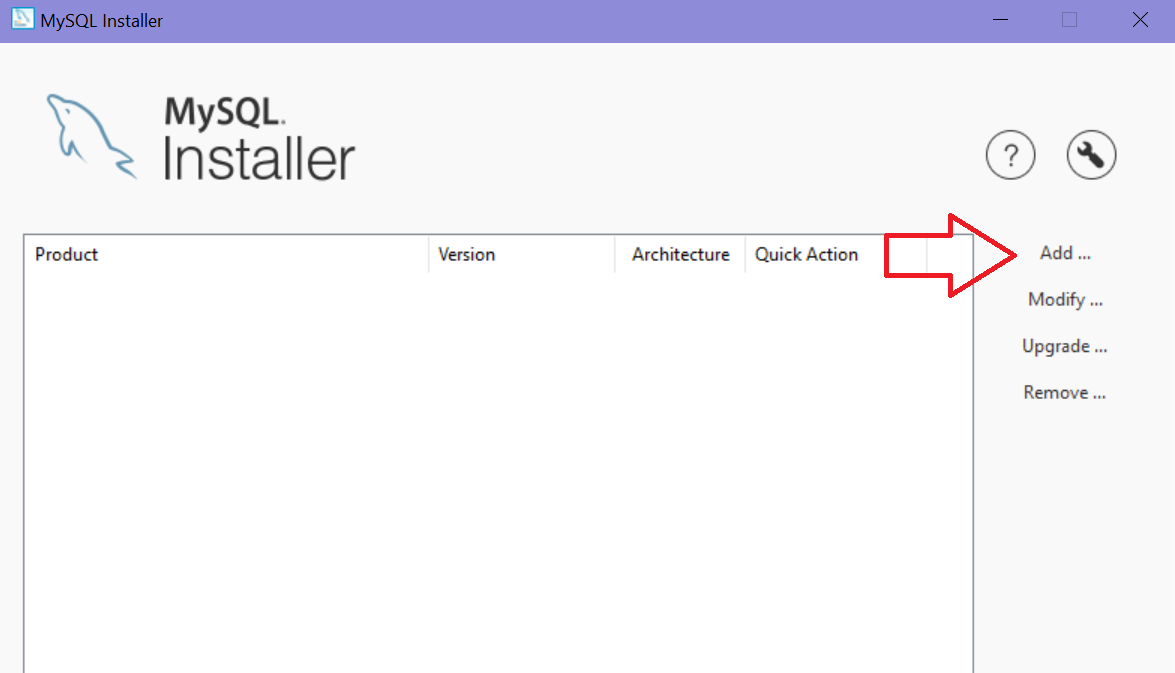
\includegraphics[width=\textwidth]{Images/mysqlinstaller.png}
\caption{\label{fig:myi} Click on the Add button}
\end{figure} 
\begin{figure}[h]
\centering
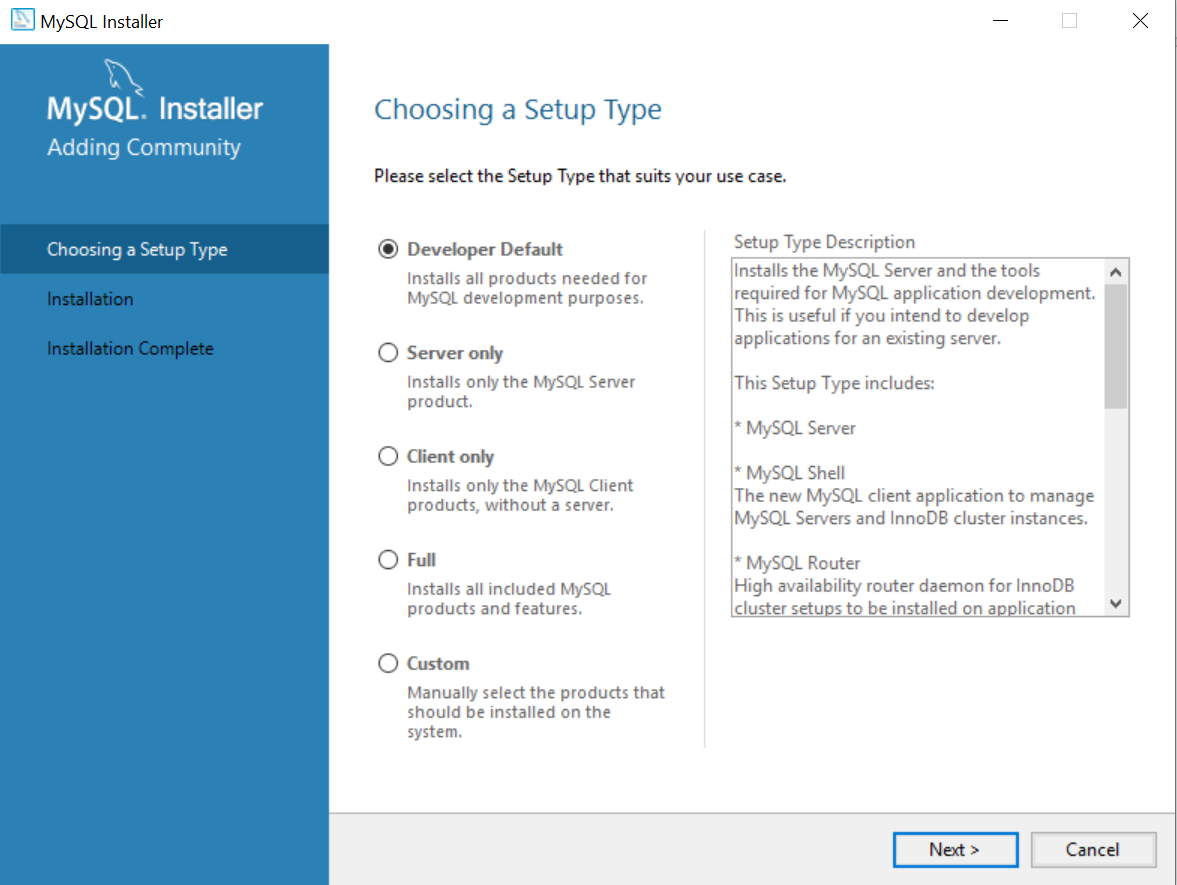
\includegraphics[width=\textwidth]{Images/mysql-download.png}
\caption{\label{fig:fmy} select Server only}
\end{figure} 
\begin{figure}[h]
\centering
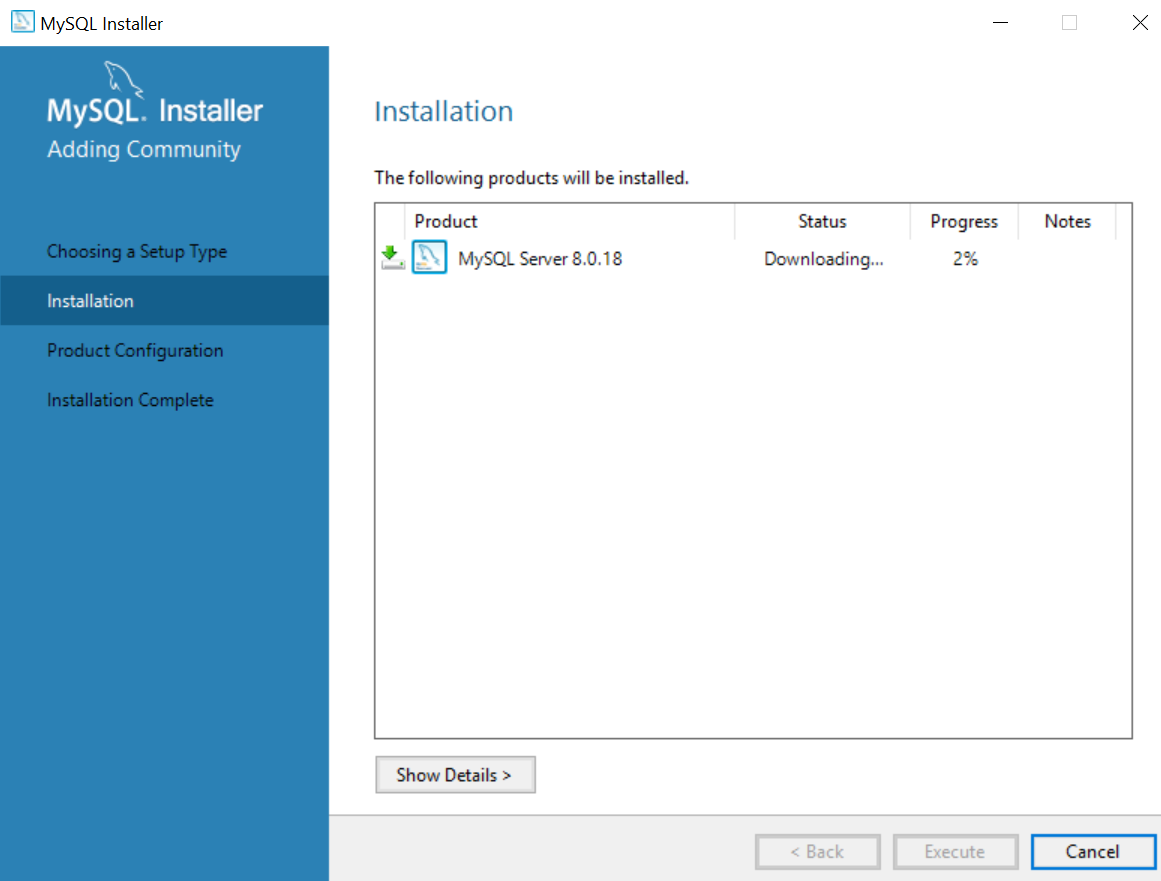
\includegraphics[width=\textwidth]{Images/mysql-downloading.png}
\caption{\label{fig:fmy} click execute. After the download is complete go to product configuration}
\end{figure} 
\begin{figure}[h]
\centering
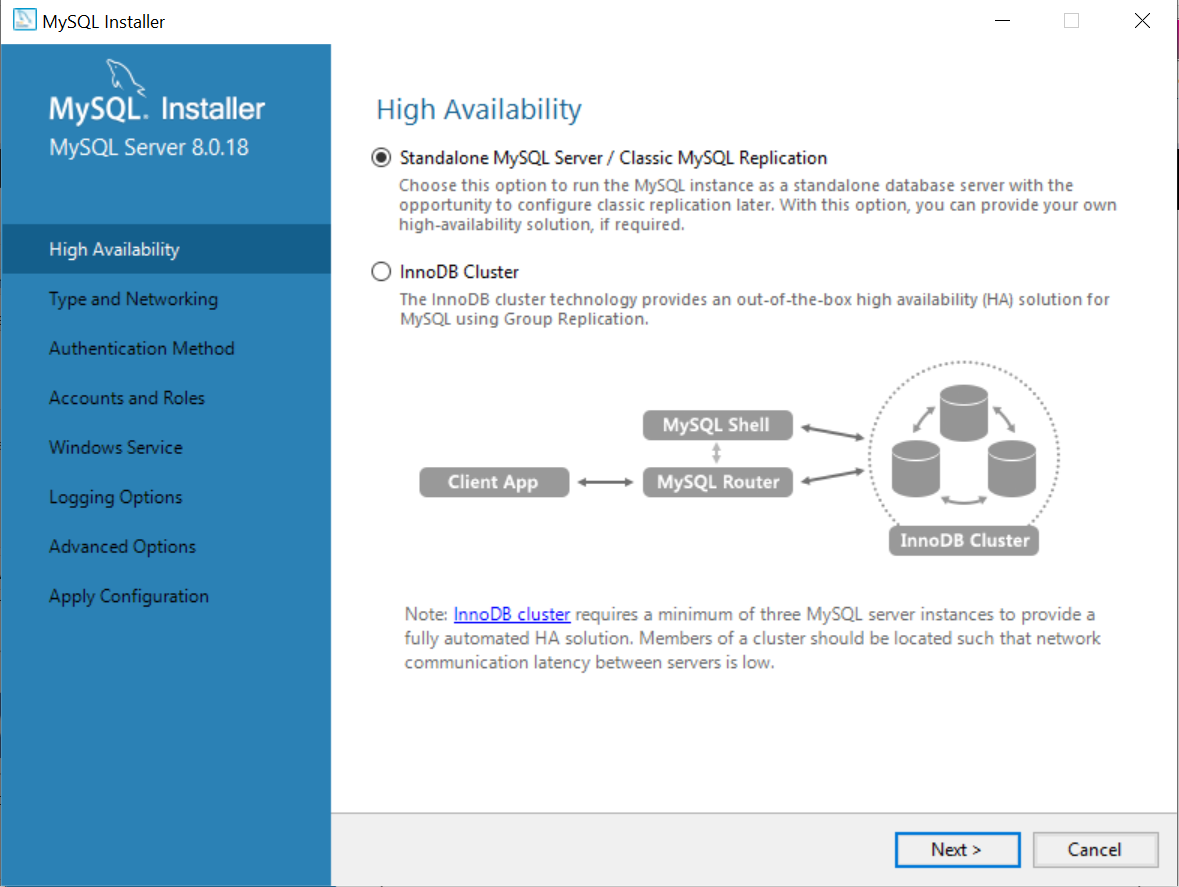
\includegraphics[width=\textwidth]{Images/first-mysql.png}
\caption{\label{fig:fmy} select Standalone MySQL Server  and then click Next }
\end{figure} 
\begin{figure}[h]
\centering
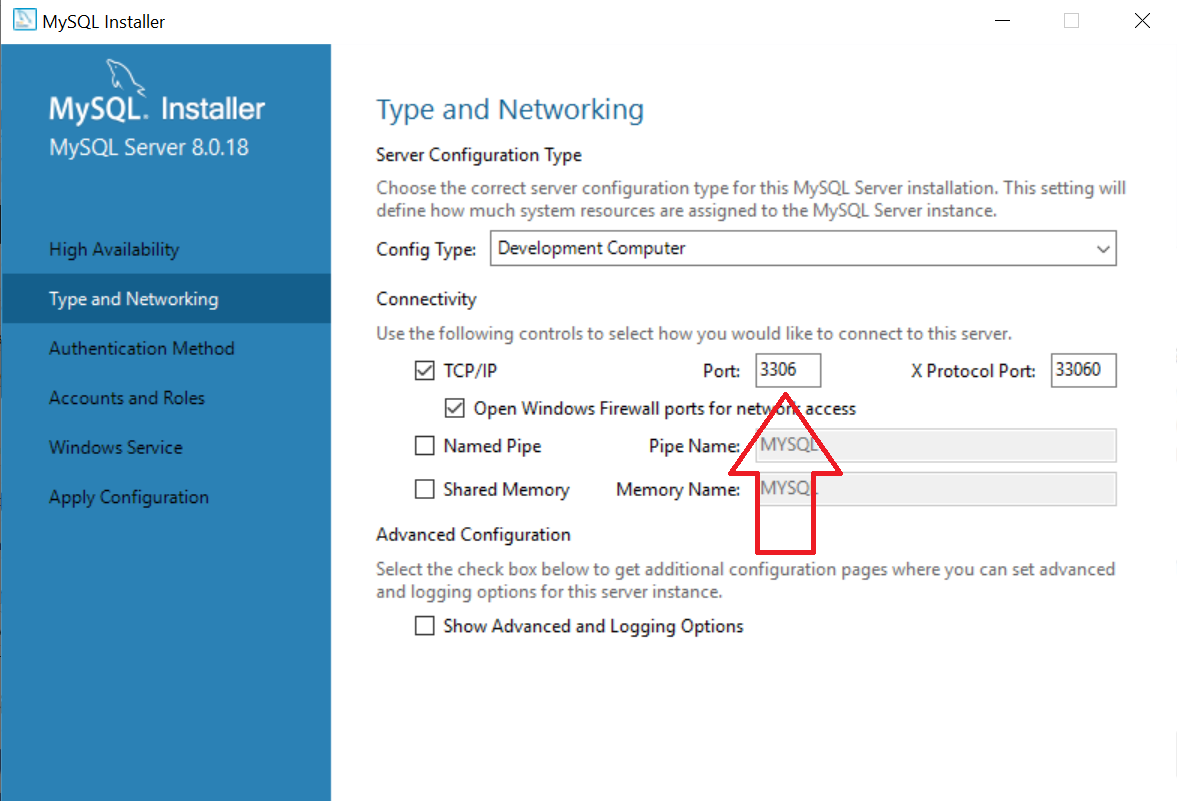
\includegraphics[width=\textwidth]{Images/second-mysql.png}
\caption{\label{fig:fmy} Check if the informations shown are the same. If you change port remember the number you insert to change later change our application setting. Click Next.Choose an authentication method. Click next.}
\end{figure} 

\begin{figure}[h]
\centering
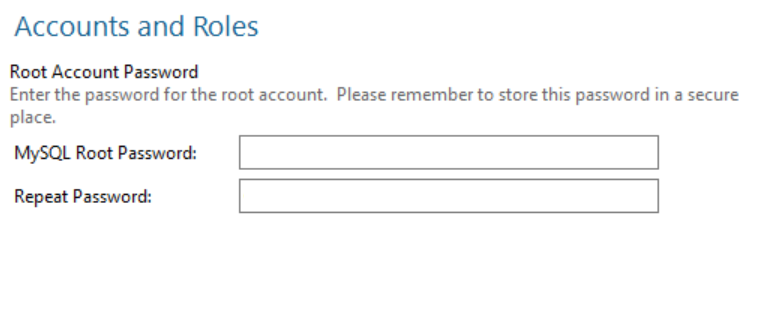
\includegraphics[width=\textwidth]{Images/4-mysql.png}
\caption{\label{fig:fmy} Set a password for the mysql server. Click next.}
\end{figure}
\begin{figure}[h]
\centering
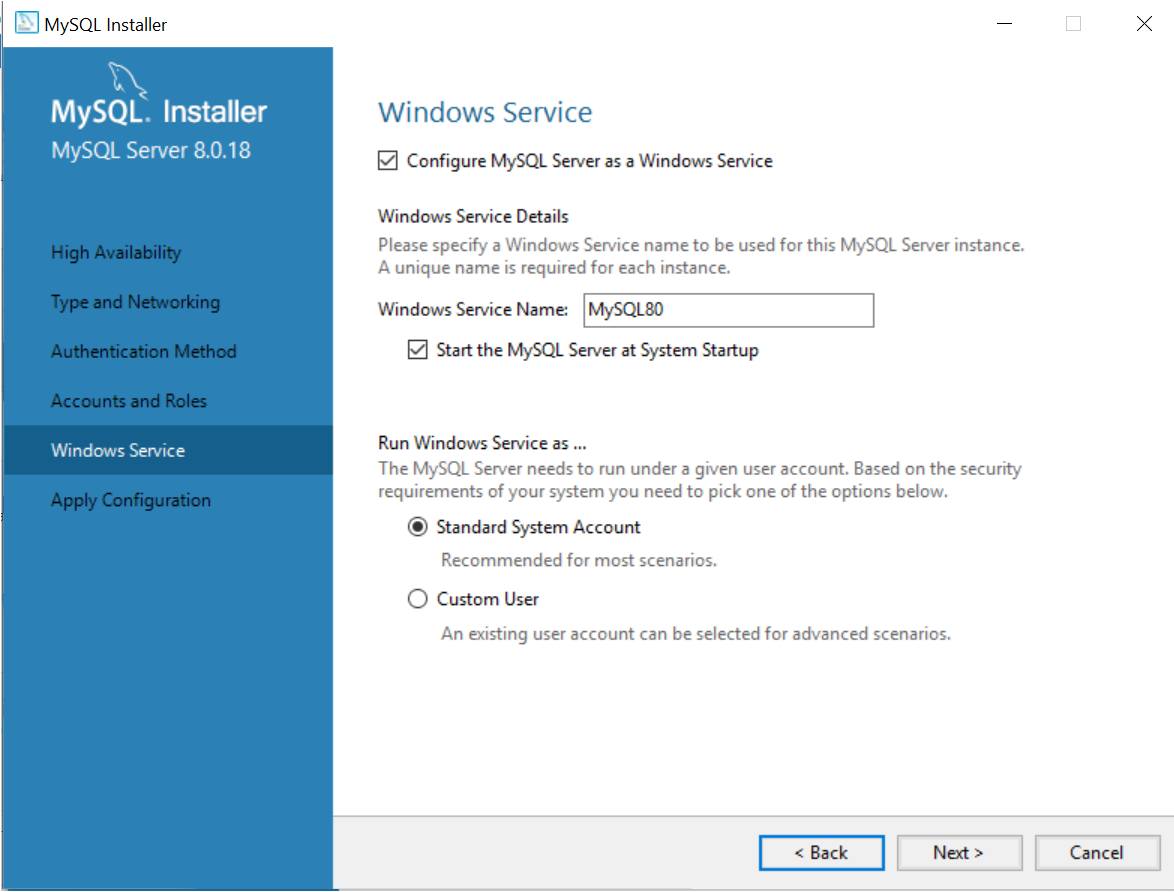
\includegraphics[width=\textwidth]{Images/6-mysql.png}
\caption{\label{fig:fmy} Click next}
\end{figure}
\begin{figure}[h]
\centering
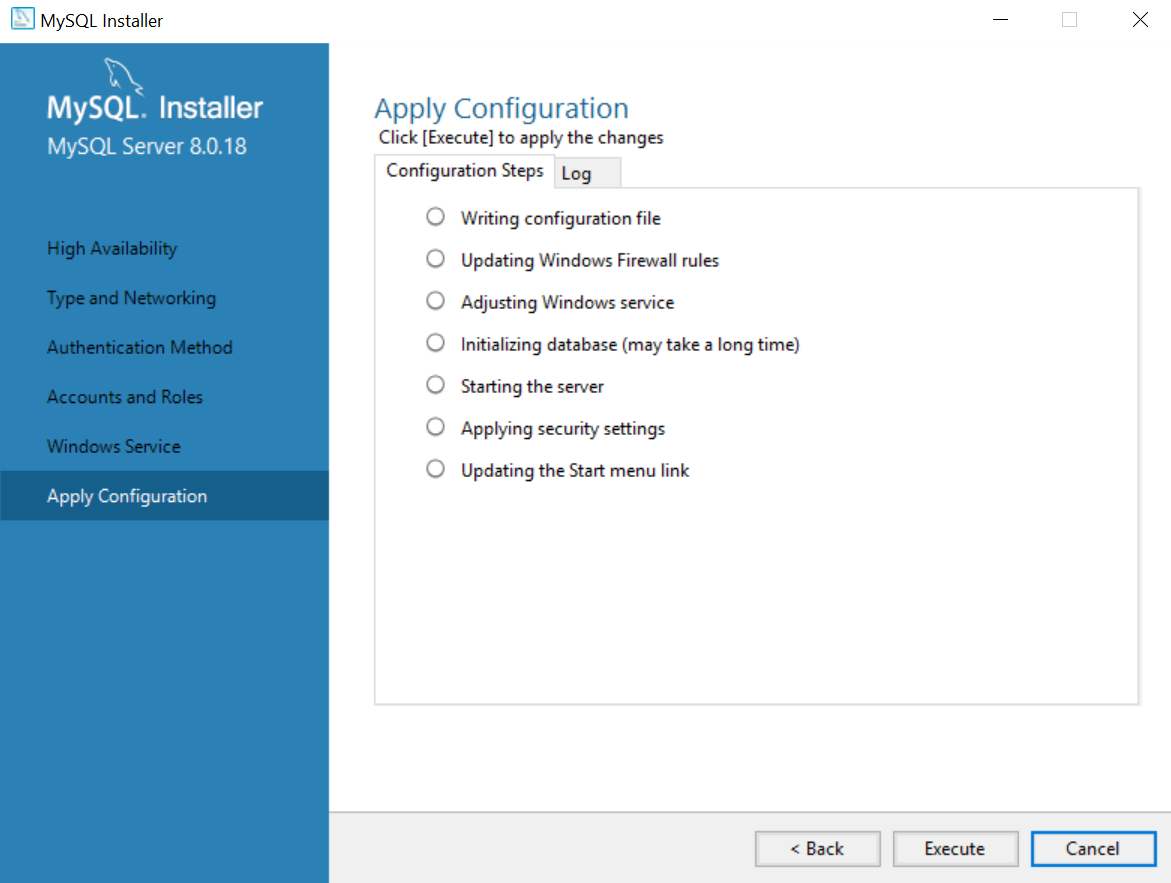
\includegraphics[width=\textwidth]{Images/7-mysql.png}
\caption{\label{fig:fmy} Click execute and after the configuration is complete click next.Your installation should be complete.
Type in your search bar mysql you should get an entry called mysql 8.0 command line client open it and insert the password you have chosen for mysql. You should now be able to use my sql server on your pc.}
\end{figure}


\clearpage
\subsection{Configure SafeStreets}
From our directory get the DB.sql file and paste it inside the bin directory that you can find inside the mysql installation forlder.
You should find the folder inside your program folder.
Now open mysql command line client. Once you log in type the commands  
\newline 
\newline create schema safestreets;
\newline use safestreets; 
\newline source DB.sql;.
\newline
\newline 
Don't forget the semicolon(;) at the end of the commands.
This should install the database. Try the command \newline select * from authority;  
\newline if a table is returned than the import is successful.

After this open the configuration.txt file in our directory.
Don't delete the text on the left part and always keep at least a white space between left part and right part.
Set the variables to the correct values. 
Set Db\_username to the username you use to connect to mysql(if you didn't choose any write root) , db\_password to the password you use to connect to the database. If you changed port for mysql server during the installation change the number 3306 with the chosen port in db\_url mail\_username and mail\_password are used to send email to the account which registers to our service. you may put there your gmail account username and password (but only if you don't have a 2 factor authentication enabled, we suggest you to keep the account which is already there)
Server Address should remain unchanged ,  if you modify tomcat configuration and change port please change it also here.
Photo path represents the path were the photos are saved. If you want change it to desired folder (which must be accessible for both read and write operations).
If you want to check what issues happens when running the code keep verbose true  otherwise change true with false. Once you modified the configuration.txt put it in the tomcat  folder.
Now put the SafeStreets.war file from our directory in the webapps folder. Now executing the startup.bat or startup.sh from the bin folder of tomcat the server should be working.
For a first check go to webapps folder and see if along with the SafeStreets app there is now a SafeStreets folder. After that open a browser search  http://localhost:8080/SafeStreets/ you should be seeing now our homepage.
On tomcat console some setup messages are shown if any error occures check out if there are errors printed there.
Whenever you want to stop the server execute the shutdown.bat or shutdown.sh in the bin folder of tomcat and the server will go oflline.
To Start testing you can get some accounts credentials executing from mysql command line the commands.
\newline 
\newline
use safestreets; 
\newline
select * from user;
\newline 
\newline
You may register as a new Citizen from the login and registration page. Other users can be registered only by other users. Authorities only by municipality. Municipality only from municipalities and Managers . Managers only by managers.
 

%------------------------------------------------------------------------------------------------------------------------------------------------




\end{document}
